% Bellwether paper. Build with `make` or `tectonic main.tex` in this directory,
% or with `tectonic paper/main.tex` from the repository root.
%
% balance=false, pbalance=true: acmart's default end-of-document column
% balancing (balance.sty) silently drops floats deferred to the last page;
% pbalance balances the last page without that failure.
\documentclass[sigconf,nonacm,balance=false,pbalance=true]{acmart}

\usepackage{array}
\usepackage{tikz}
\usetikzlibrary{arrows.meta,positioning,calc,shapes.geometric}
% Shared style for every data-driven results panel.
%
% Each results panel is a pgfplots template that reads one CSV file in data/,
% written by `bellwether report --paper` from ledger records; data/README.md
% fixes the schema of every file. A panel whose file does not exist is drawn
% as a framed placeholder (figures/pending.tex). Plot and placeholder occupy
% the same fixed box, so pagination does not change when data arrives.
\usepackage{pgfplots}
\usepackage{pgfplotstable}
\pgfplotsset{compat=1.18}
\usepgfplotslibrary{colorbrewer,fillbetween}

% Palette. One family, ColorBrewer, checked for color-vision deficiency:
% categorical slots are Dark2 hues reordered so that adjacent slots stay
% distinct under protanopia and deuteranopia, and the first three slots stay
% pairwise distinct, for the scatter plot; every slot has at least 3:1
% contrast on white. Ordered stages use a one-hue Blues ramp, magnitudes the
% Blues colormap, and signed quantities the RdBu colormap with blue for fewer
% bytes and red for more. Every series also has its own marker and dash
% pattern, so no plot depends on color alone, in print or in grayscale.
\definecolor{bwA}{HTML}{1B9E77}% teal
\definecolor{bwB}{HTML}{D95F02}% orange
\definecolor{bwC}{HTML}{7570B3}% purple
\definecolor{bwD}{HTML}{A6761D}% brown
\definecolor{bwE}{HTML}{E7298A}% magenta
\definecolor{bwStageA}{HTML}{6BAED6}% Blues, light
\definecolor{bwStageB}{HTML}{2171B5}% Blues, middle
\definecolor{bwStageC}{HTML}{08306B}% Blues, dark
\definecolor{bwInk}{HTML}{252525}
\definecolor{bwGrid}{HTML}{DDDDDD}
\definecolor{bwAxis}{HTML}{8C8C8C}

% Panel geometry. A panel is \linewidth wide and #1 tall. The axis rectangle
% sits inside it with margins #2 (left), #3 (bottom), #4 (right), and #5 (top,
% where the legend or colorbar goes, outside the data area). The bwpanel
% environment clips everything it draws to the panel, so a long label can
% never run into a neighboring panel, and fixes its bounding box to the panel.
\pgfplotsset{
  bw box/.style n args={5}{
    scale only axis, anchor=south west, at={(#2,#3)},
    width=\linewidth-#2-#4, height=#1-#3-#5,
    legend style={xshift=(#4-#2)/2}},
}
% (TikZ stops counting paths toward the picture size after a \clip, which
% leaves a pgfplots axis with an empty box; the box is fixed at the end
% anyway, so counting is switched back on.)
\makeatletter
\newenvironment{bwpanel}[1]{%
  \def\bwpanelheight{#1}%
  \begin{tikzpicture}
  \clip (0,0) rectangle (\linewidth,#1);
  \pgf@relevantforpicturesizetrue}{%
  \pgfresetboundingbox
  \path[use as bounding box] (0,0) rectangle (\linewidth,\bwpanelheight);
  \end{tikzpicture}}
\makeatother

% Tables: comma-separated, header row, and `#` lines for provenance.
\pgfplotstableset{col sep=comma, comment chars={\#}}

% Axis style shared by every panel: 6pt type, light solid grid, thin gray
% axis lines, ticks outside on the left and bottom, and the legend above the
% axis rectangle, outside the data area, so it can never cover a point.
\pgfplotsset{
  bw/.style={
    font=\scriptsize,
    every tick label/.append style={font=\scriptsize, text=bwInk},
    every axis label/.append style={font=\scriptsize, text=bwInk},
    legend style={font=\scriptsize, text=bwInk, draw=none, fill=none,
      at={(0.5,1)}, anchor=south, inner sep=0.5pt, outer sep=0pt,
      /tikz/every even column/.append style={column sep=3pt}},
    legend cell align=left,
    legend image post style={mark size=1.2pt},
    legend image code/.code={%
      \draw[mark repeat=2, mark phase=2, ##1]
        plot coordinates {(0cm,0cm) (0.2cm,0cm) (0.4cm,0cm)};},
    grid=major, major grid style={bwGrid, line width=0.3pt},
    axis line style={bwAxis, line width=0.4pt},
    tick style={bwAxis, line width=0.4pt},
    major tick length=2pt, minor tick length=1pt,
    tick align=outside, tick pos=left,
    xlabel style={inner sep=1pt}, ylabel style={inner sep=1pt},
    every axis plot/.append style={line width=0.75pt},
    mark size=1.2pt,
    unbounded coords=discard,
  },
  % Lookup strategies: one color, marker, and dash pattern each, the same in
  % every figure.
  bw index/.style={bwA, solid, mark=*, mark options={solid}},
  bw stats/.style={bwB, dashed, mark=square*, mark options={solid}},
  bw datafusion/.style={bwC, dash dot, mark=diamond*, mark options={solid}},
  bw duckdb/.style={bwD, densely dotted, mark=triangle*, mark options={solid}},
  bw raw/.style={bwE, loosely dashed, mark=pentagon*, mark options={solid}},
  % A horizontal colorbar above the axis, 80% of its width, with its tick
  % scale factor (for example 10^9) to the right of the bar, inside the panel.
  bw colorbar/.style={
    colorbar horizontal,
    colorbar style={at={(0,1.04)}, anchor=south west, height=0.12cm,
      width=0.8*\pgfkeysvalueof{/pgfplots/parent axis width},
      xticklabel pos=upper, font=\scriptsize,
      every x tick scale label/.style={at={(1,0.5)}, anchor=west,
        inner sep=1.5pt, font=\scriptsize}}},
  % A compact legend swatch for bars.
  bw bar legend/.style={legend image code/.code={%
    \fill[##1, draw=none] (0cm,-0.07cm) rectangle (0.3cm,0.07cm);}},
  % Keep only the rows whose column #1 equals #2; other rows are discarded.
  bw only/.style 2 args={
    x filter/.code={%
      \edef\bwcell{\thisrow{#1}}\edef\bwwant{#2}%
      \ifx\bwcell\bwwant\else\def\pgfmathresult{nan}\fi}},
  % Colormaps. Magnitude: ColorBrewer Blues from its third step, so the low
  % end stays visible on white. Signed: ColorBrewer RdBu, blue for negative,
  % near-white at zero, red for positive.
  /pgfplots/colormap={bwblues}{rgb255=(198,219,239) rgb255=(158,202,225)
    rgb255=(107,174,214) rgb255=(66,146,198) rgb255=(33,113,181)
    rgb255=(8,81,156) rgb255=(8,48,107)},
  /pgfplots/colormap={bwdiverging}{rgb255=(33,102,172) rgb255=(103,169,207)
    rgb255=(209,229,240) rgb255=(247,247,247) rgb255=(253,219,199)
    rgb255=(239,138,98) rgb255=(178,24,43)},
}

% Position of a lookup strategy on a categorical axis, from its key in the
% data; an unknown key maps outside the axis and is discarded, not an error.
\makeatletter
\def\bw@pos@raw{0}\def\bw@pos@stats{1}\def\bw@pos@duckdb{2}%
\def\bw@pos@datafusion{3}\def\bw@pos@index{4}%
\newcommand{\bwstrategypos}[1]{%
  \ifcsname bw@pos@#1\endcsname\csname bw@pos@#1\endcsname\else -100\fi}
\makeatother

% Labels read from data are typeset literally: while a panel reads its file,
% _ & $ ^ ~ are ordinary characters (data/README.md lists what a label may
% not contain).
\newcommand{\bwdatacatcodes}{%
  \catcode`\_=12 \catcode`\&=12 \catcode`\$=12 \catcode`\^=12 \catcode`\~=12 }

% \bwloglimits{<file>}{<column>}{<column>} sets \bwlo and \bwhi to half the
% least and twice the greatest value in the two columns, so that a log-log
% plot can use one range on both axes and its corner-to-corner line is y = x.
\newcommand{\bwloglimits}[3]{%
  \pgfplotstableread{#1}\bwtable
  \gdef\bwmin{}\gdef\bwmax{}%
  \pgfplotstableforeachcolumnelement{#2}\of\bwtable\as\bwcell{\bwtrack}%
  \pgfplotstableforeachcolumnelement{#3}\of\bwtable\as\bwcell{\bwtrack}%
  \begingroup
    \pgfkeys{/pgf/fpu=true, /pgf/fpu/output format=sci}%
    \pgfmathparse{\bwmin/2}\xdef\bwlo{\pgfmathresult}%
    \pgfmathparse{\bwmax*2}\xdef\bwhi{\pgfmathresult}%
  \endgroup}
\newcommand{\bwtrack}{%
  \begingroup
    \pgfkeys{/pgf/fpu=true, /pgf/fpu/output format=sci}%
    \ifx\bwmin\empty
      \pgfmathparse{\bwcell}\xdef\bwmin{\pgfmathresult}\xdef\bwmax{\pgfmathresult}%
    \else
      \pgfmathparse{min(\bwmin,\bwcell)}\xdef\bwmin{\pgfmathresult}%
      \pgfmathparse{max(\bwmax,\bwcell)}\xdef\bwmax{\pgfmathresult}%
    \fi
  \endgroup}

% \bwsymlimit{<file>}{<column>} sets \bwabs to the greatest absolute value in
% the column, ignoring nan, so that a diverging colormap is centered on zero.
\newcommand{\bwsymlimit}[2]{%
  \pgfplotstableread{#1}\bwtable
  \gdef\bwabs{1}%
  \pgfplotstableforeachcolumnelement{#2}\of\bwtable\as\bwcell{%
    \begingroup
      \pgfkeys{/pgf/fpu=true, /pgf/fpu/output format=sci}%
      \pgfmathfloatparsenumber{\bwcell}%
      \pgfmathfloatgetflagstomacro\pgfmathresult\bwflag
      \ifnum\bwflag<3
        \pgfmathparse{max(\bwabs,abs(\bwcell))}\xdef\bwabs{\pgfmathresult}%
      \fi
    \endgroup}}

% \bwlatencyseries{<strategy key>}{<legend label>}: inside an axis, the p50
% line of one strategy from data/latency.csv, with a band and a whisker from
% p50 to p95 (the whisker keeps p95 visible when only one rung exists).
\newcommand{\bwlatencyseries}[2]{%
  \addplot[name path=bwlat#1lo, draw=none, mark=none, forget plot,
    bw only={strategy}{#1}] table[x=files, y=p50_ms] {data/latency.csv};
  \addplot[name path=bwlat#1hi, draw=none, mark=none, forget plot,
    bw only={strategy}{#1}] table[x=files, y=p95_ms] {data/latency.csv};
  \addplot[bw #1, draw=none, mark=none, fill opacity=0.15, forget plot]
    fill between[of=bwlat#1lo and bwlat#1hi];
  \addplot[bw #1, bw only={strategy}{#1},
      error bars/.cd, y dir=plus, y explicit,
      error bar style={solid, line width=0.4pt}, error mark=none]
    table[x=files, y=p50_ms, y error plus expr=\thisrow{p95_ms}-\thisrow{p50_ms}]
    {data/latency.csv};
  \addlegendentry{#2}}

% \bwmaxint{<file>}{<column>} sets \bwlast to the greatest value in an
% integer column, for example the last row index of a heatmap, so that its
% ticks are exactly 0 to \bwlast.
\newcommand{\bwmaxint}[2]{%
  \pgfplotstableread{#1}\bwtable
  \gdef\bwlast{0}%
  \pgfplotstableforeachcolumnelement{#2}\of\bwtable\as\bwcell{%
    \ifnum\bwcell>\bwlast\relax\xdef\bwlast{\bwcell}\fi}}

\usepackage{newfloat}
\usepackage{algpseudocode}
\usepackage{enumitem}
\usepackage{subcaption}

% Algorithm float declared with newfloat (avoids algorithm.sty).
\DeclareFloatingEnvironment[name=Algorithm,placement=tbp]{algorithm}

% \todo{...}: a visible margin note marking something the author must check,
% for example a citation that could not be fully verified against a primary
% source. Use only in running text (not inside floats, captions, or tables).
\setlength{\marginparsep}{4pt}
\setlength{\marginparwidth}{40pt}
\newcommand{\todo}[1]{\textcolor{red}{\textsuperscript{\textdagger}}%
  \marginpar{\raggedright\tiny\sffamily\textcolor{red}{TODO: #1}}}

% Framed placeholder for a results panel whose data does not exist yet.
% Every results panel is drawn by pgfplots from a CSV file in data/ that
% `bellwether report --paper` writes from ledger records (data/README.md);
% until that file exists the panel is drawn as this frame. The frame fills
% exactly the box the plot will occupy, \linewidth wide and <height> tall, so
% pagination does not change when the data arrives.
%
% Usage: \pendingfigure[<font size>]{<height>}{<what the panel will show>}{<file>}
% where <file> is the CSV file name in data/ without its extension.
\newcommand{\pendingfigure}[4][\footnotesize]{%
  \begin{tikzpicture}
    \draw[thick, rounded corners=2pt, fill=black!3]
      (0.4pt,0.4pt) rectangle (\linewidth-0.4pt,#2-0.4pt);
    \node[text width=\linewidth-14pt, align=center, font=#1]
      at (0.5\linewidth,0.5*#2)
      {Figure pending: #3, drawn from \texttt{data/#4.csv}, which
       \texttt{bellwether report -{}-paper} writes from ledger records};
    \pgfresetboundingbox
    \path[use as bounding box] (0,0) rectangle (\linewidth,#2);
  \end{tikzpicture}%
}


% References to the project's design documents, which are cited once as
% \cite{bellwether}: decision records as ADR NNN, other documents by file name.
\newcommand{\adr}[1]{ADR~#1}
\newcommand{\doc}[1]{\texttt{#1}}
\newcommand{\code}[1]{\texttt{#1}}
\newcommand{\Eq}{\mathrm{Eq}}
\newcommand{\RG}{\mathcal{G}}
\newcommand{\pend}{pending}
% Breakable underscore for long identifiers in narrow columns.
\newcommand{\us}{\_\allowbreak}

% Let TeX stretch interword space before it overfills a narrow column.
\setlength{\emergencystretch}{1.5em}

\begin{document}

\title[Bellwether]{Bellwether: Reflective Optimization of Data Pipelines with
  an Exact Counterfactual Loss and Reconciliation Certificates}

\author{Vincent Pham}
\affiliation{\institution{Independent}\city{}\country{}}

\begin{abstract}
Index advisors for relational databases depend on the optimizer's what-if
interface, which estimates the cost of a hypothetical index. These estimates are
often wrong: configurations recommended by large language models, which look
worse by estimated cost, can run faster than an industrial tuner's. Data lakes
have no optimizer of their own and so no exact what-if interface, which has kept
both classical and LLM-driven tuning out of the storage tier where much
analytical data now lives. We observe that this absence is an opportunity.
Because a lake exposes its files, the I/O cost of a hypothetical index,
composite key, or plan over those files can be computed exactly, with no
estimation, by replaying the workload's recorded key sets against file and
row-group metadata. We present Bellwether, which (i) builds row-group-level
secondary indexes with composite and temporal keys over Parquet, (ii) provides
an exact counterfactual what-if interface, (iii) runs a reflective,
population-based optimizer over plans, physical designs, and whole pipelines,
using counterfactual attribution as its backward pass, exact finite-difference
descent for numeric knobs, and Pareto selection across recorded runs, and (iv)
certifies every change by index-accelerated reconciliation at the pipeline
output, producing equivalence certificates where SQL provers cannot apply and
admitting non-local rewrites across step boundaries. A language model proposes;
only the engine scores, verifies, and applies, and every step is a
content-addressed record. Evaluation on a synthetic versioned-ledger benchmark
with planted anti-patterns is pending.
\end{abstract}

% CCS concepts: placeholder, to be regenerated with the ACM CCS tool
% (https://dl.acm.org/ccs) before submission.
\ccsdesc[500]{Information systems~Autonomous database administration}
\ccsdesc[300]{Information systems~Query optimization}
\ccsdesc[100]{Information systems~Data access methods}

\keywords{index advisors, what-if analysis, data lakes, Parquet, query
  rewriting, equivalence verification, reconciliation, LLM agents, reflective
  optimization, Pareto selection}

\maketitle

\section{Introduction}\label{sec:intro}

An index advisor chooses indexes for a workload by asking, for each candidate
configuration, what every query would cost if that configuration existed.
Relational systems answer with the optimizer's what-if interface, which costs a
query against hypothetical indexes that are never built~\cite{whatif1998}, and
advisors search over configurations with that interface as their
oracle~\cite{autoadmin1997,bruno2005relax,kossmann2020}. The oracle is an
estimate. Cardinality estimates in industrial optimizers are routinely and
substantially wrong~\cite{leis2015}, and optimizer estimates often predict that
an index will help a query that it in fact slows down~\cite{aimeetsai}. A recent
study on SQL Server found that index configurations recommended by large
language models, which often look worse than the industrial tuner's under the
optimizer's estimated cost, in several cases ran faster in actual execution,
although their quality varied widely~\cite{dtallm2026}. An advisor that ranks by
estimate can be outperformed by one that ignores the estimate.

Much analytical data now lives as open columnar files, typically Parquet, in
object storage, read by several engines rather than owned by
one~\cite{lakehouse2021}. Table formats record per-file statistics for data
skipping~\cite{deltalake,icebergspec}, and indexing subsystems add secondary
indexes for particular engines, in one case with what-if analysis over
hypothetical indexes inside that engine's optimizer~\cite{hyperspace}. The
storage tier itself has no optimizer, and so no what-if interface that every
engine reading the files can share, and none that is exact. Classical advisors
therefore have no engine-independent oracle there, and language-model tuners
have nothing trustworthy to be scored against.

We observe that this absence is an opportunity. A lake exposes its files. For
keyed workloads (look up a batch of keys, find the latest version of each key,
or find the version current at a timestamp), the I/O a run performs under a
hypothetical index depends on three things that can be recorded or read: the
run's key set, the row groups that contain each key, and the compressed size of
each row group. Replaying a recorded workload against row-group metadata
therefore computes, rather than estimates, the bytes, row groups, and files each
run would read under a candidate key specification (\adr{005}). We call this an
exact counterfactual what-if interface. Its exactness is scoped: it covers I/O
over files that exist, so a hypothetical layout is costed exactly only once it
is materialized, and costs above the scan come from measured execution
(Section~\ref{sec:exact}).

An exact oracle also changes what can be trusted from a language model.
LLM-based rewriters~\cite{genrewrite,llmr2,lithe,quite,e3rewrite,resequel}
generate candidates that must be scored and checked. Scoring by estimate
inherits the problem above. Checking with an equivalence
prover~\cite{cosette,qed,sqlsolver,verieql} covers restricted SQL fragments,
while pipeline steps are written in Spark, KQL, Scala, and configuration
(\adr{004}), and many useful changes are not query rewrites at all: an index, a
layout, a lookback bound. Bellwether therefore gives the model no authority. A
model may observe and propose; only the engine may measure, verify, and apply
(\adr{009}). The verifier is reconciliation of the pipeline's output over the
keys the workload touched (\adr{004}). This paper makes five contributions.

\begin{enumerate}[leftmargin=*,label=\textbf{C\arabic*}]
  \item \textbf{An exact counterfactual what-if interface for lakes.} Replay
    of recorded key sets against row-group metadata yields the exact I/O cost of
    hypothetical key specs (including composite and temporal keys) and plans
    over existing files; zero estimation error is a falsifiable design property
    (Section~\ref{sec:whatif}).
  \item \textbf{Reconciliation certificates.} Index-accelerated reconciliation
    by latest version, canonical row hash, and exact decimal totals yields
    certificates with an explicit coverage statement where SQL provers cannot
    apply; gating at the pipeline output admits non-local rewrites
    (Section~\ref{sec:cert}).
  \item \textbf{A hybrid proposer loop.} A reflective, population-based
    optimizer over plans, designs, and pipelines uses counterfactual attribution
    as its backward pass, a language model for structure, exact
    finite-difference descent for knobs, rule-driven enumeration, and Pareto
    selection across runs (Section~\ref{sec:evolve}).
  \item \textbf{A validated rulebook.} Distilled rules are promoted only when
    held-out replay reproduces a gain and the gate passes
    (Section~\ref{sec:rulebook}).
  \item \textbf{A trust boundary and a replayable ledger.} Every step is a
    content-addressed record, nothing a proposer emits is a score, and a search
    replays from its ledger byte for byte (Sections~\ref{sec:overview}
    and~\ref{sec:determinism}).
\end{enumerate}

This paper describes a fixed, documented design~\cite{bellwether} and a system
under construction; we cite design documents by file name and decision records
as ADR~001 to ADR~025. The contract, source, and ledger crates are merged, the
index core and two further crates are in review, and the optimizer is planned
(Section~\ref{sec:impl}). The evaluation methodology was fixed before any
implementation (\adr{019}); Section~\ref{sec:eval} reports it in full and marks
every result as pending. The paper's claims are therefore design properties,
each tied to a design document or an invariant with a named test, and none is a
measurement.

\section{Background and Related Work}\label{sec:related}

\paragraph{Index advisors and the what-if interface.} AutoAdmin introduced
cost-driven index selection that stays in step with the
optimizer~\cite{autoadmin1997} and the what-if interface that costs hypothetical
indexes without building them~\cite{whatif1998}. Later work replaced bottom-up
heuristics with a relaxation-based search~\cite{bruno2005relax}, and an
experimental study compares index selection algorithms~\cite{kossmann2020}. All of them score candidates with optimizer
estimates. Estimation errors are large and routine~\cite{leis2015}; one
response replaces optimizer-based plan comparison inside tuners with a
classifier trained on executions~\cite{aimeetsai}. Language models now act as
advisors: LLMIA uses in-context demonstrations and database
feedback~\cite{llmia}, AMAZe coordinates zero-shot agents~\cite{amaze}, and
EvoTune tunes knobs, query hints, and indexes together with a memory of past
tuning feedback~\cite{memtuning}. Bellwether addresses a narrower class of
decisions than a relational advisor, keyed I/O over lake files, and in exchange
removes the estimate from that class.

\paragraph{LLM query rewriting.} GenRewrite guides a model with natural-language
rewrite rules and repairs its output in a counterexample-guided
loop~\cite{genrewrite}. LLM-R\textsuperscript{2} has a model select rules for
a conventional rule-based rewriter~\cite{llmr2}. LITHE combines prompt
ensembles, database-aware prompts, and search guided by token probabilities,
and applies logic-based and statistical checks before it shows a
rewrite~\cite{lithe}. QUITE coordinates training-free agents with live database
feedback~\cite{quite}. E3-Rewrite trains a rewriter by reinforcement learning
with rewards for executability, equivalence, and efficiency~\cite{e3rewrite}.
ReSequel turns catalog metadata into template-specific rules for the model and
checks candidate rewrites on sampled data~\cite{resequel}. Each rewrites SQL
queries individually and judges a rewrite by optimizer estimates, execution, or
checks on data. Evolve differs in three respects: it searches against a
recorded workload with a loss that is exact for I/O; it selects by Pareto
dominance over runs rather than by one score; and its artifacts include
indexes, layouts, knobs, and multi-step pipelines, gated at the pipeline output.

\paragraph{Equivalence verification.} Cosette combines constraint solving with
an interactive proof assistant~\cite{cosette}. SQLSolver reduces equivalence to
linear integer arithmetic extended with unbounded sums~\cite{sqlsolver}.
VeriEQL proves or refutes bounded equivalence under integrity constraints and
returns counterexamples~\cite{verieql}. QED decides equivalence under bag
semantics for a defined fragment~\cite{qed}. EquiTrace builds equivalence
proofs from an optimizer's rewrite rules~\cite{equitrace}, and Narasayya and
Chaudhuri use the optimizer's own machinery to check the soundness of LLM-based
rewrites on real workloads~\cite{narasayya2026verify}. These tools establish
equivalence for all instances within a SQL fragment. Reconciliation checks one
property, output equality over a stated key scope, for any language and for
changes that are not rewrites (Section~\ref{sec:provers}); the two compose.

\paragraph{Layouts and data skipping.} Small materialized aggregates skip blocks
using per-block summaries~\cite{moerkotte1998sma}. Workload-aware partitioning
groups tuples so that queries skip blocks~\cite{sun2014skipping}; Qd-tree learns
a routing tree for records from a workload~\cite{qdtree}; MTO optimizes block
layouts jointly across tables that are joined~\cite{ding2021layouts}; LRP
builds partitions that are robust to shifts in the query
distribution~\cite{lrp2025}; and WAIR reclusters only the micro-partitions that sit
on query-range boundaries~\cite{recluster2026}. These methods choose layouts.
Evolve treats a layout as one candidate among keys and knobs, costs it exactly
once it is materialized, and gates it by reconciliation.

\paragraph{Lake indexing.} Delta Lake records per-file minimum and maximum
statistics in its log and uses them to skip files~\cite{deltalake}, and
Iceberg's manifests carry per-file column bounds for scan
planning~\cite{icebergspec}. Parquet embeds split-block Bloom filters hashed
with XXH64~\cite{parquetbloom}, a blocked design that follows Putze et
al.~\cite{putze2007}. Hyperspace builds secondary indexes over lake files for
Spark in Azure Synapse, and its paper describes what-if analysis and index
recommendation over hypothetical indexes within that engine's
optimizer~\cite{hyperspace}. Apache Hudi maintains bloom, record-level, and column-statistics indexes inside its table format~\cite{hudi}, and ClickHouse offers data-skipping indexes (min/max, set, and bloom variants) over granules inside the engine~\cite{clickhouse}; Parquet itself carries a page index and optional bloom filters~\cite{parquetbloom}. Each is coupled to a table format or an engine, none runs over plain files from a single process, and none advises which key to index. Learned Bloom
filters trade a model for filter space~\cite{plbf2021,plbf2410,cascadedlbf}; they
are a deferred research direction for Bellwether (\doc{work-packages.md}).
Bellwether's index kinds are not new. What it adds is an exact what-if interface
that no single engine owns, certificates, and a boundary between a proposer and
the engine that scores it.

\paragraph{Text-space optimization.} ProTeGi~\cite{protegi} and
TextGrad~\cite{textgrad} improve prompts and other text with natural-language
feedback treated as a gradient. DSPy compiles declarative pipelines of
language-model calls~\cite{dspy}, and MIPRO optimizes their instructions and
demonstrations~\cite{mipro}. GEPA evolves prompts by reflection and draws
candidates from the Pareto frontier of its own attempts~\cite{gepa}. SkillOpt
edits an agent's skill document and accepts an edit only if it improves a
held-out validation score~\cite{skillopt}. Evolve borrows the reflective,
population-based loop, Pareto selection, and the validation gate, and makes
three substitutions (\adr{021}): an exact replay replaces the benchmark score,
counterfactual attribution replaces credit assignment inferred by the model,
and a hard equivalence gate replaces an optional check.

\section{System Overview}\label{sec:overview}

Bellwether is a standalone engine for folders of Parquet files; CSV and
JSON-lines files are read by treating fixed byte-range chunks as row groups, so
nothing above the source layer sees the difference (\doc{format.md}). It
explains why a keyed query read more than it returned, proposes a change from
exact measurement, and attests that the change returns the same rows
(\doc{architecture.md}). It does not execute queries. It emits a scan plan, a
superset of the row groups that hold the queried keys together with a residual
predicate, and an engine such as DuckDB, DataFusion, or Spark reads the rows
(\adr{011}).

\subsection{The boundary and the loop}\label{sec:loop}

One sentence governs the design (\doc{architecture.md}): \emph{the agent may
observe and propose; only the engine may measure, verify, and apply; and
nothing crosses from the first side to the second without a content-addressed
record of why.} Figure~\ref{fig:loop} shows the four stages.
(1)~\emph{Observe}: an agent or a human reads Evidence, such as fanout per
column (the files and row groups one value touches, at p50, p95, and max),
lints from the rule catalog, a workload summary, or a scan plan; observe tools
are read-only, cache-backed, make no network calls, and have a 100\,ms budget.
(2)~\emph{Propose}: the agent writes a Proposal, which is a key specification,
a layout, or a rewrite described as data (before shape, after shape, invariant).
The Proposal type has no score field, so a score cannot be injected
(\doc{threat-model.md}). (3)~\emph{Score and verify}: the engine replays the
recorded workload under the current configuration and under the proposal and
writes a Replay of per-run costs (Section~\ref{sec:whatif}); it then builds the
candidate, runs the job both ways, reconciles the outputs, and writes a
Certificate (Section~\ref{sec:cert}). (4)~\emph{Apply and attest}: the engine
refuses unless the Certificate passed and was computed against the current
manifest, applies the change, and only then writes a Receipt that links the
chain and records the manifest sequence before and after (invariant~2).

The command-line interface and the Model Context Protocol (MCP)
server~\cite{mcpspec} share one code path, so humans and agents see identical
evidence (\adr{010}). MCP tools come in three tiers that follow the stages,
\code{observe.*}, \code{propose.*}, and \code{apply.*}, and \code{apply.*}
accepts only a Certificate id.

\begin{figure*}[t]
  \centering
  % The four-stage loop and the trust boundary (docs/architecture.md).
% Redrawn from the README's loop figure (now docs/assets/readme/loop-light.svg,
% drawn by scripts/render_figures.py). Used in a figure* environment.
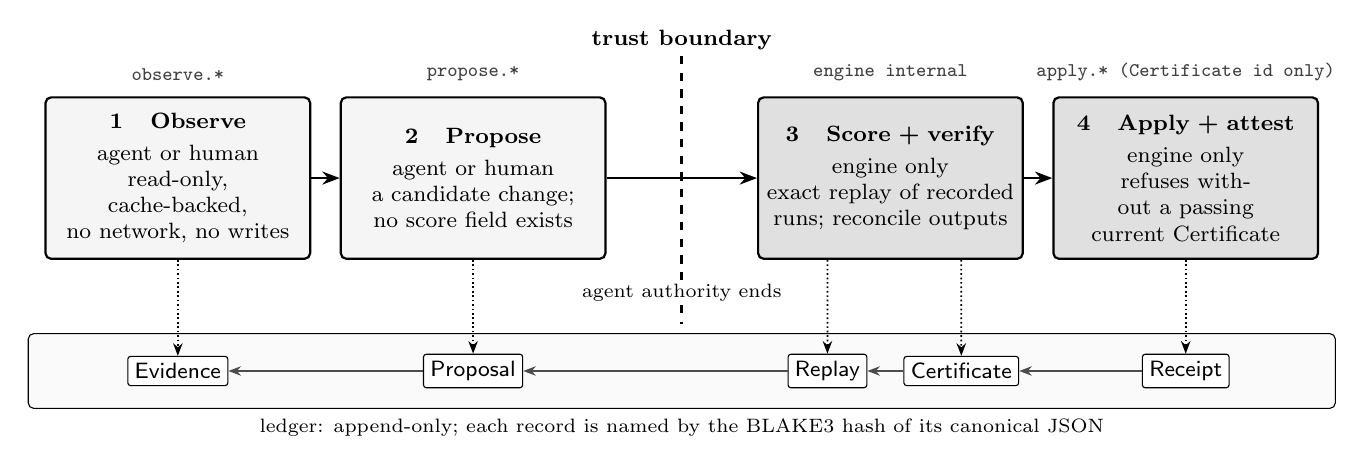
\begin{tikzpicture}[
    font=\footnotesize,
    stage/.style={draw, thick, rounded corners=2pt, text width=3.15cm,
                  minimum height=2.05cm, align=center, inner sep=3pt},
    agent/.style={stage, fill=black!4},
    engine/.style={stage, fill=black!12},
    rec/.style={draw, rounded corners=1pt, fill=white, inner sep=2.5pt,
                font=\footnotesize\sffamily},
    tier/.style={font=\scriptsize\ttfamily, text=black!75},
    flow/.style={-{Stealth[length=2.2mm]}, thick},
    walk/.style={-{Stealth[length=1.6mm]}, semithick, black!70},
    drop/.style={-{Stealth[length=1.6mm]}, semithick, densely dotted},
  ]
  % Stages.
  \node[agent]  (obs) at (0.0,0) {\textbf{1\quad Observe}\\[2pt]
      agent or human\\ read-only, cache-backed,\\ no network, no writes};
  \node[agent]  (pro) at (3.75,0) {\textbf{2\quad Propose}\\[2pt]
      agent or human\\ a candidate change;\\ no score field exists};
  \node[engine] (sco) at (9.05,0) {\textbf{3\quad Score + verify}\\[2pt]
      engine only\\ exact replay of recorded\\ runs; reconcile outputs};
  \node[engine] (app) at (12.8,0) {\textbf{4\quad Apply + attest}\\[2pt]
      engine only\\ refuses without a passing\\ current Certificate};

  % Interface tiers.
  \node[tier, above=2pt of obs] {observe.*};
  \node[tier, above=2pt of pro] {propose.*};
  \node[tier, above=2pt of sco] {engine internal};
  \node[tier, above=2pt of app] {apply.* (Certificate id only)};

  % Flow between stages.
  \draw[flow] (obs) -- (pro);
  \draw[flow] (pro) -- (sco);
  \draw[flow] (sco) -- (app);

  % Trust boundary.
  \draw[dashed, very thick] (6.4,1.55) -- (6.4,-1.85);
  \node[font=\footnotesize\bfseries, fill=white, inner sep=1pt] at (6.4,1.75)
      {trust boundary};
  \node[font=\scriptsize, fill=white, inner sep=1pt, align=center] at (6.4,-1.45)
      {agent authority ends};

  % Ledger band and the records each stage writes.
  \node[draw, rounded corners=2pt, fill=black!2, minimum width=16.6cm,
        minimum height=0.95cm] (ledger) at (6.4,-2.45) {};
  \node[font=\scriptsize, anchor=north] at (ledger.south)
      {ledger: append-only; each record is named by the BLAKE3 hash of its canonical JSON};
  \node[rec] (ev)   at (0.0,-2.45)  {Evidence};
  \node[rec] (pr)   at (3.75,-2.45) {Proposal};
  \node[rec] (rp)   at (8.25,-2.45) {Replay};
  \node[rec] (ce)   at (9.95,-2.45) {Certificate};
  \node[rec] (rc)   at (12.8,-2.45) {Receipt};
  \draw[drop] (obs.south) -- (ev.north);
  \draw[drop] (pro.south) -- (pr.north);
  \draw[drop] (sco.south) ++(-0.8,0) -- (rp.north);
  \draw[drop] (sco.south) ++(0.9,0) -- (ce.north);
  \draw[drop] (app.south) -- (rc.north);

  % Order in which a reviewer walks back from a Receipt.
  \draw[walk] (rc) -- (ce);
  \draw[walk] (ce) -- (rp);
  \draw[walk] (rp) -- (pr);
  \draw[walk] (pr) -- (ev);
\end{tikzpicture}

  \caption{The four-stage loop and the trust boundary, after
    \doc{docs/architecture.md}. Stages 1 and 2 are open to an agent; stages 3
    and 4 run only inside the engine. Every stage writes a record to the
    ledger. Arrows inside the ledger show the order in which a reviewer walks
    back from a Receipt to the Evidence it rests on.}
  \Description{Four boxes in a row: Observe and Propose on the agent side,
    Score plus verify and Apply plus attest on the engine side, separated by a
    dashed vertical line labeled trust boundary. Each box writes a record into
    a ledger band below: Evidence, Proposal, Replay and Certificate, Receipt.}
  \label{fig:loop}
\end{figure*}

\subsection{Records, ledger, and threat model}\label{sec:ledger}

Every record is canonical JSON named by the BLAKE3 hash~\cite{blake3} of its
bytes and stored append-only (\adr{006}); field order is part of the hash, and
every record carries a version (\doc{format.md}). The current contract,
implemented as Rust types, has five records: Evidence, Proposal, Replay,
Certificate, and Receipt, and only the engine writes the last three. Evidence
and Certificates carry provenance (input hashes, the age of the oldest input, a
creation time, and the manifest version when one exists; invariant~6), so a
stale measurement cannot pass as fresh. Because
records link by hash, a reviewer or a continuous integration gate reads one
Receipt and can check every step behind it.

The threat model claims that a compromised, confused, or hallucinating agent
can waste time by proposing bad ideas and can do nothing else
(\doc{threat-model.md}). No tool accepts a file path to write, a shell command,
or a query string to execute, because rewrites are data and never code the
engine runs. The engine never consults a model for a score, a verification
outcome, or an apply decision (\adr{009}, as amended). Content addressing makes
tampering detectable but not preventable until records are signed, and an
attacker with write access to the store is out of scope.

\subsection{Storage, crates, and invariants}\label{sec:storage}

The engine's state lives beside the data: immutable segments named by their
content hash, a manifest committed by conditional PUT, the ledger, and a
rebuildable cache (\doc{format.md}, \adr{003}). A writer that loses the
conditional PUT re-reads the manifest, unions its segments with the winner's,
and retries, so readers never block (\adr{015}). The manifest carries a
sequence number that increases by one per commit, and replays and receipts
reference manifests by it (\adr{020}). Crate dependencies point one way: the
index core and the source readers know nothing above them
(Section~\ref{sec:impl}). Table~\ref{tab:invariants} lists the six invariants;
each is paired with a test that fails if it stops holding
(\doc{invariants.md}).

\begin{table}[t]
  \caption{Invariants and the crates that enforce them, from
    \doc{docs/invariants.md}.}
  \label{tab:invariants}
  \small
  \begin{tabular}{@{}r>{\raggedright\arraybackslash}p{0.62\columnwidth}l@{}}
    \toprule
    \# & Invariant & Crate \\
    \midrule
    1 & No false negatives in pruning: a row group that holds a queried key is
        in the scan plan, on every index path. & core \\
    2 & A Receipt implies a passing Certificate computed against the manifest
        it was applied to. & ledger \\
    3 & Replay is deterministic: same manifest, workload, and proposal give a
        byte-identical Replay. & replay \\
    4 & Readers see one manifest version while a build commits. & store \\
    5 & A temporal lookup never returns a superseded row. & core \\
    6 & Evidence and Certificates carry provenance: inputs, age, and creation
        time; a Certificate also names its manifest. & ledger, profile \\
    \bottomrule
  \end{tabular}
\end{table}

\section{An Exact Counterfactual What-If Interface}\label{sec:whatif}

\subsection{Model}\label{sec:model}

\paragraph{Files and row groups.} A file is identified by a fingerprint (path,
size, etag or modification time, and a BLAKE3 hash of its last 64\,KiB or,
under a stricter policy, of the whole file), not by its path, so an in-place
rewrite is detected as drift (\doc{format.md}). Each
row group receives a dense 32-bit id at the first sighting of (fingerprint,
position in file); ids are never reused, and drift tombstones the old ids
(\adr{013}). Let $\RG$ be the live row-group ids, $f(g)$ the file of row group
$g$, and $b(g)$ its compressed size from the file footer. For
$G \subseteq \RG$ let $f(G) = \{ f(g) : g \in G \}$.

\paragraph{Key specs and selections.} A key spec is $\mathsf{Exact}$ or
$\mathsf{Bloom}$ over a column list (bloom adds a target false-positive rate),
$\mathsf{Range}$ over one column, or $\mathsf{Temporal}$ over a column list
with a timestamp column. A composite key is a column list longer than one,
encoded so that byte order equals typed order and each element is
self-delimiting, so a probe on a prefix of leading elements seeks every
extension (\adr{002}, \adr{016}). For a spec $s$ and a probe $k$, the selection $S_s(k) \subseteq \RG$
is the set of row groups the index returns: for $\mathsf{Exact}$, those holding
a row whose key starts with $k$; for $\mathsf{Bloom}$, those whose filter
accepts $k$, a superset of exact membership; for $\mathsf{Range}$, those whose
minimum and maximum bound the probed value or interval; for $\mathsf{Temporal}$,
those holding a version of $k$ at its greatest timestamp (\emph{latest}) or at
the greatest timestamp not after $t$ (\emph{as-of} $t$), ties included
(\doc{format.md}). Footer statistics and embedded bloom filters alone give a
baseline selection $S_\varnothing(k)$. Let $T(k)$ be the row groups that must
be read to answer $k$ exactly. Invariant~1 requires $T(k) \subseteq S_s(k)$ on
every path. For temporal probes this needs the index-wide maximum timestamp per
key, consulted before ranking, so a superseded row is never returned even when
the newest version sits in a row group pruned for another reason
(invariant~5). Null timestamps rank last and never win (\adr{014}).

\paragraph{Runs and cost.} A recorded run $r$ carries its key set $K_r$, its
query kind (locate, latest, or as-of), and parameters such as an as-of
timestamp. Under spec $s$ it reads $G_s(r) = \bigcup_{k \in K_r} S_s(k)$, and
its cost is the vector of bytes, row groups, and files, which are the fields of
a \code{RunCost} record:
\begin{equation}\label{eq:cost}
  c_s(r) \;=\; \Big( \textstyle\sum_{g \in G_s(r)} b(g),\;\; |G_s(r)|,\;\;
  |f(G_s(r))| \Big).
\end{equation}
A physical design $D$ is a set of specs; let $D_r \subseteq D$ be the specs
whose leading columns run $r$ binds. Each selection contains $T(k)$, so their
intersection does too, and the engine intersects bitmaps over the global id
space (\adr{001}):
\begin{equation}\label{eq:design}
  G_D(r) = \textstyle\bigcap_{s \in D_r} G_s(r), \qquad
  G_D(r) = G_\varnothing(r) \text{ if } D_r = \emptyset .
\end{equation}

\subsection{Why the cost is exact}\label{sec:exact}

\emph{Design property.} $c_D(r)$ is computed without an estimated quantity.
$K_r$ is recorded. Each $S_s(k)$ is a deterministic function of the files: key
membership for exact and temporal specs, filter bits for bloom specs (fixed by
the canonical encoding and the hash function; \adr{008}, \adr{016}), and footer
bounds for range specs. $b(g)$ is read from the footer. There is no cardinality
estimate, cost model, or sampling, and the same workload, manifest, and
proposal yield a byte-identical Replay (invariant~3). The predicted quantity is
also the one the plan prescribes: a consumer that executes the scan plan reads
the row groups in $G_D(r)$ and applies the residual predicate (\adr{011}).

Three boundaries keep the claim precise, and the paper's use of ``exact'' is
narrowed to them. (1)~\emph{I/O as accounted by row-group metadata}: $b(g)$ is
a row group's total compressed size, a consumer that projects columns reads a
subset of it, and per-column chunk sizes are not yet in the statistics type
(\doc{rule-catalog.md}), so projection savings are outside the exact cost, as
are reads of footers, segments, and the manifest. (2)~\emph{Files that exist}:
a hypothetical key spec over existing files is exact, but a hypothetical layout
changes the row-group statistics, which do not exist until the layout is
written. Its cost is exact once the layout is materialized, and until then no
number is reported, because \code{RunCost} has no field for an estimate
(\doc{rule-catalog.md}, \code{scattered\us time\us column}). (3)~\emph{Scans whose
key sets are recorded or derived from the run's inputs}, such as trigger keys
and parameters: costs above the scan (CPU, memory, latency) and scans whose key
sets depend on unrecorded intermediate results are measured by an attached
executor through the planned \code{Scorer} trait, not replayed
(\doc{evolve.md} \S10).

\subsection{Computing a counterfactual}\label{sec:counterfactual}

A counterfactual asks what a recorded run would have read under a design that
differs from the current one. Range specs and the statistics baseline need only
footers. For an exact, bloom, or temporal spec that has not been built, replay
constructs a transient in-memory segment from a projected read of the key
columns (and the timestamp column for temporal specs), one segment at a time
(\doc{work-packages.md}, \adr{018}). The read is paid once per column set and
shared by every run and every candidate over those columns; each run then costs
one lookup per key, one bitmap union, and one sum.

Prefix seek models subsumption: an exact spec on $(a, b)$ answers a probe on
$a$ alone, so for runs keyed by $a$ it replaces a spec on $a$. Nulls are handled
per tuple (\adr{014}, as amended): a tuple is indexed when its leading column is
non-null, a null in a trailing column is encoded with the null marker so the
tuple stays prefix-seekable, and a probe containing a null matches nothing, as
in SQL's three-valued logic. The composite's prefix selection therefore equals
the single-column selection, including rows whose trailing columns are null, so
dropping the single-column spec preserves invariant~1.

\subsection{Index structures and complexity}\label{sec:segments}

Segments are immutable and content-addressed, and each indexes one key spec
over a range of row-group ids (\doc{format.md}). An exact segment stores sorted
key blocks, a split-block bloom filter per block~\cite{parquetbloom}, and for
each key a roaring bitmap~\cite{roaring} over global row-group ids
(\adr{001}). A temporal segment adds, per key, a chain of (timestamp, row group)
pairs and the key's maximum timestamp. A bloom segment stores one split-block
filter per row group, the shape Parquet embeds, and records whether a filter
hashes canonical bytes or Parquet's plain encoding so that a probe is encoded
to match (\adr{008}, amendment). A range segment stores a minimum and maximum
per row group. One canonical byte encoding per Arrow type serves ordering,
bloom hashing, and the row hashing of Section~\ref{sec:cert} (\adr{016}).
Adding a key spec builds segments over every row group and records completeness
in the manifest; a query on an incomplete spec fails rather than returning a
partial answer (\adr{012}).

For a segment with $n$ distinct keys, an exact lookup of key set $K$
binary-searches the block index, probes one block's filter, and searches that
block's key directory only if the filter passes, for $O(|K| \log n)$
comparisons, while holding one block index and the bitmaps of the keys asked
(\adr{018}). The union is proportional to the bitmaps' containers and the byte
sum is $O(|G_D(r)|)$. Building a transient segment is one projected pass over
the key columns, with memory bounded by one segment (\doc{format.md}).
The design budget for one replay of one run under one candidate is 5\,ms on the
medium synthetic dataset (\doc{evolve.md} \S12); the harness asserts it, and it
is a budget, not a measurement.

\section{Reconciliation Certificates}\label{sec:cert}

Reconciliation is the verifier (\adr{004}). It checks equivalence on data
rather than on syntax, so it applies to changes that no SQL prover accepts, and
it states exactly which keys it checked.

\subsection{The verifier}\label{sec:verifier}

Reconciliation compares a left output $L$ (the baseline) with a right output
$R$ (the candidate) by key. Its parameters are the key columns, an optional
latest-by column, ignored columns, and group and decimal columns for totals.
For each key $k$ in a scope $Q$ it takes the latest-version rows of $k$ on each
side, $L_k$ and $R_k$ (the rows at $k$'s greatest latest-by value; null
timestamps never win, \adr{014}), and compares them by a row hash $h$: xxh3-128
from the xxHash family~\cite{xxhash} over the canonical encodings of the
non-ignored columns in schema order, each preceded by its column name's length
and bytes, with an explicit null marker (\doc{format.md}, \adr{016}). It also
sums decimal columns per group exactly, at the dataset's declared scale. The
Certificate records
\begin{align*}
  \mathit{missing\_right} &= |\{ k \in Q : L_k \neq \emptyset,\ R_k = \emptyset \}|,\\
  \mathit{missing\_left}  &= |\{ k \in Q : L_k = \emptyset,\ R_k \neq \emptyset \}|,\\
  \mathit{mismatched}     &= |\{ k \in Q : L_k, R_k \neq \emptyset,\
                              h(L_k) \neq h(R_k) \}|,
\end{align*}
the ignored columns, and every group whose totals differ, with both totals at
the declared scale. It passes if and only if the three counts are zero and no
totals differ (\doc{agent-loop.md}). The index makes this cheap (\adr{004}):
the scope of a workload certificate is the set of keys the recorded runs
touched, and the index locates them to row groups, so running the job both ways
and reconciling reads the row groups that hold touched keys rather than the
dataset.

\subsection{Coverage}\label{sec:coverage}

Every Certificate states its coverage: \emph{full} (every key),
\emph{workload} (the keys of a named recorded workload, with their count), or
\emph{sampled} (a number of keys and the sampled fraction).
\emph{Guarantee (design property):} a passing Certificate with scope $Q$
asserts that for every $k \in Q$ the latest-version rows of $k$ agree on every
non-ignored column, up to collisions of a 128-bit non-cryptographic hash, and
that group totals over the compared rows agree exactly. It asserts nothing
about keys outside $Q$; in the design's words, a Certificate is a statement
about the keys it covers and nothing more (\doc{agent-loop.md}).

\subsection{Why provers do not apply}\label{sec:provers}

SQL equivalence provers and deciders establish equivalence for all database
instances, or for all instances up to a bound, within a supported SQL
fragment~\cite{cosette,qed,sqlsolver,verieql}. Bellwether's changes fall outside
that setting in three ways (\adr{004}). Pipeline steps are written as Spark
plans, KQL, Scala, or configuration, which these tools do not accept. Many
changes are not query rewrites at all: a key spec, a bloom false-positive rate,
a lookback bound, a layout. And the rewrites with the largest effect often cross
step boundaries and change intermediate results
(Section~\ref{sec:nonlocal}). Reconciliation applies to all three because it
compares outputs; the price is that a Certificate covers the keys it compared,
not all inputs. The two kinds of evidence compose: where a rule catalog identity
applies, such as a semi-join on $K$ commuting with a window partitioned by $K$,
the gate may use the identity for that edit and reconciliation for the rest
(\doc{evolve.md} \S1, \S4.2). In the current contract a static identity has no
Certificate path and so cannot reach a Receipt; the planned \code{Verifier}
trait adds one (\doc{rule-catalog.md}; \doc{evolve.md} \S10).

\subsection{Whole-pipeline equivalence and non-local rewrites}\label{sec:nonlocal}

A pipeline is a DAG of steps with lineage. The rewrites that matter most cross
step boundaries: push a filter from a late step to an early one, materialize an
intermediate that two steps share, or remove a deduplication that a later step
repeats (\doc{evolve.md} \S5.3). Each changes some step's local output, so a
check that requires equivalence step by step must reject it. Bellwether gates at
the pipeline output instead: for a candidate $a$ and the baseline $a_0$,
$\Eq(a, a_0)$ holds when reconciliation of the two pipeline outputs over the
touched keys passes, and intermediate outputs may differ (\adr{023}).

\emph{Illustration.} Step two of a pipeline reads the full history of a
versioned table and keeps the newest version of each key; step five semi-joins
that result with the run's trigger keys. The candidate moves the semi-join into
step two and answers it with a temporal \emph{latest} lookup. Step two's output
now holds only the trigger keys, so a per-step check fails, yet step five's
output is unchanged for every trigger key, which is what the output certificate
checks. The candidate composes two catalog patterns,
\code{lookback\us unbounded} and \code{unprefiltered\us window}
(\doc{rule-catalog.md}), across a step boundary;
Figure~\ref{fig:schematic-pipeline} draws it.

\subsection{Limits}\label{sec:certlimits}

A non-local rewrite is certified for the keys the workload touched, not for all
inputs, so a rewrite that is wrong only on untouched keys would pass. How to
communicate this to a user who later runs an untouched key is an open question
in the design (\doc{evolve.md} \S13), and it is why a rule must be re-validated
on held-out runs before promotion (Section~\ref{sec:rulebook}). A sampled
certificate speaks only for its sample, and ignored columns are not compared,
which is why the Certificate lists them. The row hash is not cryptographic, so a
Certificate does not defend against an adversary who can craft colliding rows;
an attacker with write access to the store is already outside the threat model.
Data can also drift: each decision records the fanout evidence it depended on,
and a receipt whose evidence has drifted is flagged stale (\doc{evolve.md}
\S5.4).

\section{Evolve: Reflective Optimization with an Exact Loss}\label{sec:evolve}

Evolve is the optimizer of milestone M6, specified in \doc{evolve.md} and
\adr{021} to \adr{025}. It searches over plans, physical designs, and whole
pipelines against a recorded workload, with exact replay as its loss and
reconciliation as a hard constraint.

\subsection{Problem}\label{sec:problem}

A pipeline is a DAG of steps. Each step has a logical plan (a DAG of
operators), reads from a physical design (the indexes, layout, and numeric
knobs that exist), and runs many times with different inputs, such as a trigger
batch of keys or a date window. Let $W = \{r_1, \dots, r_n\}$ be the recorded
runs, each with its key set, parameters, and executed plan. An artifact $a$ in
the search space $A$ is a physical design, a plan, a pipeline, or a combination.
Let $c(a, r_i) \in \mathbb{R}^{m}$ be its exact cost vector on $r_i$, the I/O
quantities of Equation~\eqref{eq:cost} extended with measured latency when an
executor is attached; let $m(a)$ be the design's maintenance cost (index bytes
and build time); and let $\Eq(a, a_0)$ be the equivalence predicate of
Section~\ref{sec:nonlocal}. The problem is multi-objective and constrained
(\doc{evolve.md} \S1):
\begin{equation}\label{eq:problem}
  \min_{a \in A}\ \big\{ c(a, r_1), \dots, c(a, r_n),\ m(a) \big\}
  \quad \text{subject to} \quad \Eq(a, a_0).
\end{equation}
No scalar objective is used. Selection is Pareto over runs and objectives
(Section~\ref{sec:pareto}), so a candidate that wins at the median batch and
loses at the p95 batch cannot eliminate one that protects the tail. The loop
is borrowed from text-space optimization~\cite{gepa,skillopt,textgrad} and the
configuration search from physical design~\cite{autoadmin1997}; what is new is
pairing them with an exact loss and a prover-free constraint (\doc{evolve.md}
\S2).

\subsection{The loop}\label{sec:theloop}
\begin{figure}[t]
  \centering
  % Schematic; no measured quantities. Left: the evolve loop (Algorithm 1).
% Right: candidates on two runs, showing why mean selection drops the tail
% protector B while Pareto selection keeps it. Positions are illustrative
% only; the axes carry no scale.
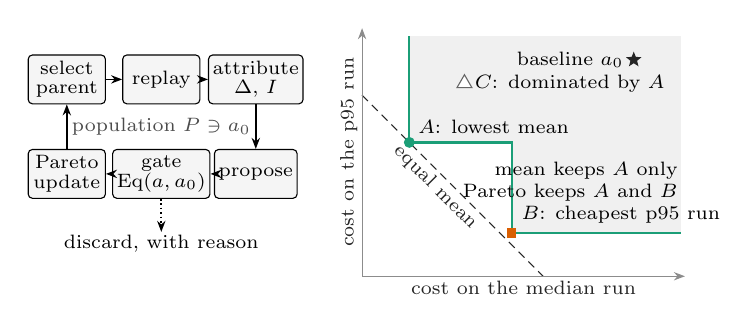
\begin{tikzpicture}[
    font=\scriptsize,
    stage/.style={draw, rounded corners=1.5pt, fill=black!4, inner sep=1.5pt,
                  minimum height=0.62cm, minimum width=0.98cm, align=center},
    flow/.style={-{Stealth[length=1.4mm]}, semithick},
  ]
  % ---- The loop.
  \node[stage] (sel) at (0.55,2.95) {select\\[-1pt]parent};
  \node[stage] (rep) at (1.75,2.95) {replay};
  \node[stage] (att) at (2.95,2.95) {attribute\\[-1pt]$\Delta$, $I$};
  \node[stage] (pro) at (2.95,1.75) {propose};
  \node[stage] (gat) at (1.75,1.75) {gate\\[-1pt]$\Eq(a, a_0)$};
  \node[stage] (upd) at (0.55,1.75) {Pareto\\[-1pt]update};
  \draw[flow] (sel) -- (rep);
  \draw[flow] (rep) -- (att);
  \draw[flow] (att) -- (pro);
  \draw[flow] (pro) -- (gat);
  \draw[flow] (gat) -- (upd);
  \draw[flow] (upd) -- (sel);
  \draw[flow, densely dotted] (gat.south) -- ++(0,-0.42)
    node[below, inner sep=1pt] {discard, with reason};
  \node[text=black!70] at (1.75,2.35) {population $P \ni a_0$};

  % ---- Two runs: cost on the median run against cost on the p95 run.
  \begin{scope}[shift={(4.3,0.45)}]
    % Region dominated by the frontier {A, B}.
    \fill[black!6] (0.6,3.05) -- (0.6,1.7) -- (1.9,1.7) -- (1.9,0.55)
      -- (4.05,0.55) -- (4.05,3.05) -- cycle;
    \draw[bwA, thick] (0.6,3.05) -- (0.6,1.7) -- (1.9,1.7) -- (1.9,0.55)
      -- (4.05,0.55);
    % Equal mean cost through A: x + y is constant along this line.
    \draw[bwInk, densely dashed] (0,2.3) -- (2.3,0);
    \node[rotate=-45, anchor=north, inner sep=1.5pt, text=bwInk]
      at (1.05,1.25) {equal mean};
    % Axes, without a scale.
    \draw[-{Stealth[length=1.4mm]}, bwAxis] (0,0) -- (4.1,0)
      node[pos=0.5, below, text=bwInk, inner sep=1.5pt] {cost on the median run};
    \draw[-{Stealth[length=1.4mm]}, bwAxis] (0,0) -- (0,3.15)
      node[pos=0.5, above, rotate=90, text=bwInk, inner sep=1.5pt]
      {cost on the p95 run};
    % Candidates.
    \node[circle, fill=bwA, inner sep=1.4pt] (A) at (0.6,1.7) {};
    \node[anchor=south west, inner sep=1.5pt] at (A.north east) {$A$: lowest mean};
    \node[fill=bwB, inner sep=1.7pt] (B) at (1.9,0.55) {};
    \node[anchor=south west, inner sep=1.5pt] at (B.north east)
      {$B$: cheapest p95 run};
    \node[draw=black!60, fill=white, regular polygon, regular polygon sides=3,
          inner sep=1.1pt] (C) at (1.3,2.45) {};
    \node[anchor=west, inner sep=1.5pt] at (C.east) {$C$: dominated by $A$};
    \node[star, star points=5, star point ratio=2.3, fill=bwInk,
          inner sep=0.9pt] (a0) at (3.45,2.75) {};
    \node[anchor=east, inner sep=1.5pt] at (a0.west) {baseline $a_0$};
    % What each rule keeps.
    \node[anchor=east, align=right, inner sep=1pt] at (4.05,1.2)
      {mean keeps $A$ only\\Pareto keeps $A$ and $B$};
  \end{scope}
\end{tikzpicture}%

  \caption{Schematic; no measured quantities. Left: the loop of
    Algorithm~\ref{alg:evolve}. Right: candidates scored on two runs. $A$ has
    the lowest mean cost, so mean selection keeps $A$ and drops $B$; $B$ is
    cheaper on the p95 run, so neither dominates the other and Pareto
    selection keeps both, $B$ as the tail protector. $A$ dominates $C$, which
    either rule drops.}
  \Description{Left, a cycle of small boxes: select parent, replay,
    attribute, propose, gate, and Pareto update, with an exit labeled discard
    at the gate. Right, a plot with unnumbered axes, cost on the median run and
    cost on the p95 run, showing the baseline, candidates A, B, and C, a
    staircase frontier through A and B over a shaded dominated region, and a
    dashed line of equal mean cost through A that passes below B.}
  \label{fig:schematic-pareto}
\end{figure}


Algorithm~\ref{alg:evolve} restates \doc{evolve.md} \S3. The baseline is always
in the population. A child that fails the gate is discarded with its reason
recorded; a child that passes is replayed and offered to the frontier. Every
step writes a ledger record, and a proposer's prompt and completion are stored
verbatim with the model identifier. Figure~\ref{fig:schematic-pareto} draws the
loop beside its selection rule.

\begin{algorithm}[t]
  \caption{Evolve (after \doc{docs/evolve.md} \S3). $W_s$ and $W_h$ are the
    search and held-out runs. Every computed value is also written to the
    ledger.}
  \label{alg:evolve}
  \small
  \begin{algorithmic}[1]
    \Require baseline $a_0$; runs $W_s$, $W_h$; rulebook $\mathcal{B}$;
      budget; seed
    \State $P \gets \{a_0\}$ \Comment{the baseline is always a member}
    \While{budget remains}
      \State $p \gets \textsc{Select}(P)$ \Comment{frontier, crowding tie-break}
      \State $\tau \gets \textsc{Replay}(p, W_s)$ \Comment{per run, per operator}
      \State $(\Delta, I) \gets \textsc{Attribute}(p, \tau)$
        \Comment{top-$k$ counterfactuals}
      \State $a \gets \textsc{Propose}(p, \tau, \Delta, I, \mathcal{B})$
        \Comment{one of three proposers}
      \If{not $\Eq(a, a_0)$}
        \State record the discard and its reason; \textbf{continue}
      \EndIf
      \State $C \gets \textsc{Replay}(a, W_s)$
      \State $P \gets \textsc{ParetoUpdate}(P, a, C)$
    \EndWhile
    \State $\mathcal{B} \gets \textsc{Distill}(\text{ledger})$, each rule
      validated on $W_h$
    \State \Return frontier of $P$, receipts, $\mathcal{B}$
  \end{algorithmic}
\end{algorithm}

\subsection{The backward pass: counterfactual attribution}\label{sec:attribution}

\begin{figure}[t]
  \centering
  % Schematic; no measured quantities. The backward pass on a small plan:
% every attributed node carries its counterfactual difference Delta, and one
% pair of choices (u, v) carries a nonzero interaction I_uv.
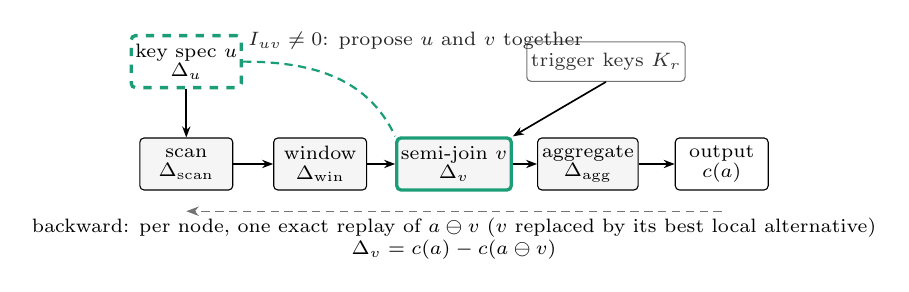
\begin{tikzpicture}[
    font=\scriptsize,
    op/.style={draw, rounded corners=1.5pt, fill=black!4, inner sep=1.5pt,
               minimum height=0.66cm, minimum width=1.18cm, align=center},
    design/.style={op, fill=white, dashed},
    input/.style={draw=black!55, rounded corners=1.5pt, inner sep=1.5pt,
                  minimum height=0.5cm, align=center, text=black!80},
    flow/.style={-{Stealth[length=1.4mm]}, semithick},
  ]
  % Operators, forward.
  \node[op] (scan) at (0.62,1.55) {scan\\[-1pt]$\Delta_{\mathrm{scan}}$};
  \node[op] (win)  at (2.32,1.55) {window\\[-1pt]$\Delta_{\mathrm{win}}$};
  \node[op, draw=bwA, very thick] (sj) at (4.02,1.55) {semi-join $v$\\[-1pt]$\Delta_v$};
  \node[op] (agg)  at (5.72,1.55) {aggregate\\[-1pt]$\Delta_{\mathrm{agg}}$};
  \node[op, fill=white] (out) at (7.42,1.55) {output\\[-1pt]$c(a)$};
  \draw[flow] (scan) -- (win);
  \draw[flow] (win) -- (sj);
  \draw[flow] (sj) -- (agg);
  \draw[flow] (agg) -- (out);
  % Inputs: a design choice and the run's trigger keys.
  \node[design, draw=bwA, very thick] (key) at (0.62,2.85) {key spec $u$\\[-1pt]$\Delta_u$};
  \node[input] (trig) at (5.95,2.85) {trigger keys $K_r$};
  \draw[flow] (key) -- (scan);
  \draw[flow] (trig.south) -- (sj.north east);
  % The interaction between u and v.
  \draw[bwA, densely dashed, thick] (key.east) to[out=0, in=115]
    (sj.north west);
  \node[anchor=south west, inner sep=1.5pt, text=bwInk] at (1.35,2.95)
    {$I_{uv} \neq 0$: propose $u$ and $v$ together};
  % The backward direction: one exact replay per node.
  \draw[-{Stealth[length=1.6mm]}, black!55, densely dashed]
    (7.42,0.95) -- (0.62,0.95);
  \node[anchor=north, inner sep=1.5pt, align=center] at (4.02,0.92)
    {backward: per node, one exact replay of $a \ominus v$ ($v$ replaced by its
     best local alternative)\\$\Delta_v = c(a) - c(a \ominus v)$};
\end{tikzpicture}%

  \caption{Schematic; no measured quantities. The backward pass on a small
    plan. Solid arrows carry data forward. Each attributed node $v$ carries
    $\Delta_v = c(a) - c(a \ominus v)$, one exact replay of $a$ with $v$
    replaced by its best local alternative. The pair $(u, v)$, a key spec and
    the semi-join, has $I_{uv} \neq 0$: a composite key that pays off only
    once the semi-join moves, so the two changes are proposed together as a
    patch set.}
  \Description{A plan drawn left to right: a key spec feeding a scan, then a
    window, a semi-join that also takes the trigger keys, an aggregate, and
    the output. Each node carries a label Delta sub v, and the output carries
    the cost c of a. A dashed arc between the key spec and the semi-join is
    labeled I sub uv not equal to zero, propose u and v together. A dashed
    arrow runs backward under the plan: one exact replay per node.}
  \label{fig:schematic-backward}
\end{figure}

A gradient says how much each parameter contributed to the loss. For a plan,
the analogue is how much each operator, and each design choice that fixed the
operator's input, contributed to the bytes read. Because replay is exact and
cheap, this is computed by counterfactual rather than approximated
(\adr{024}; Figure~\ref{fig:schematic-backward}). For an artifact $a$ and a
plan node $v$,
\begin{equation}\label{eq:attr}
  \Delta_v = c(a) - c(a \ominus v),
\end{equation}
where $a \ominus v$ replaces $v$ by its best known local alternative (the rule
catalog identity that applies there) or ablates it when none exists. For a pair
of choices $(u, v)$, with $a_u$ denoting $a$ after changing $u$,
\begin{equation}\label{eq:interaction}
  I_{uv} = c(a_{uv}) - c(a_u) - c(a_v) + c(a).
\end{equation}
Both are evaluated per run. A nonzero $I_{uv}$ means the two choices do not
compose additively, the signal that they must be proposed together as a patch
set. Attribution costs one replay per node and the interaction matrix one per
pair. It is capped at the top $k$ nodes by cost rather than sampled, because
sampling would reintroduce estimation, and Shapley values over all subsets were
rejected as exponential (\adr{024}). The design budget for attributing a
20-node plan is one second (\doc{evolve.md} \S12).

\subsection{Three proposers, and what ``gradient'' means}\label{sec:proposers}

The artifacts are discrete: text, DAGs, and sets. There is no differentiable
path from a plan to its cost, so calling the loop gradient descent without
qualification would be inaccurate (\adr{022}). Evolve uses three substitutes
with one scorer and one gate.

\paragraph{Textual gradients for structure.} For operator order, join strategy,
keys, and layouts, the proposer is a language model given the parent, its
per-run trace, its attribution, and the rulebook, and asked for a critique and
one mutation. The critique is a textual gradient in the sense of
ProTeGi~\cite{protegi} and TextGrad~\cite{textgrad}, and the mutation is the
update step. The difference is that the critique is grounded in $\Delta_v$: the
model is told which operator cost what instead of inferring it. Mutations are
plan edits that name an identity when one applies (for example,
\code{semijoin\us before\us window}), so the gate can use a static proof for that
edit and reconciliation for the rest.

\paragraph{Exact numeric descent for knobs.} Numeric knobs include bloom
false-positive rates, key-count gates (when to broadcast, push an \code{IN}
list, or fall back to a shuffle), lookback windows, chunk and segment sizes, and
partition counts. Cost is a deterministic function of them, so the central
difference $\big(c(\theta + h e_j) - c(\theta - h e_j)\big)/2h$ has no
sampling noise, only discretization error, and coordinate descent, pattern
search, and integer line search apply without variance reduction. This is the
one part of evolve that is literally gradient-like, and it is limited to knobs.
Following Section~\ref{sec:exact}, knobs that change what is read from existing
files (rates, gates, lookbacks) are replayed exactly at every probe, while knobs
that change the files (partition counts, and chunk sizes for text sources) are
exact only once each probed point is materialized. Because a proposer's output
is only a candidate, the scalar that descent follows, such as bytes on one
template's p95 run, need not match the selection rule: every point descent
visits is scored on the full objective matrix and gated like any other.

\paragraph{Rule-driven enumeration and deferred surrogates.} The rule catalog's
detectors produce deterministic candidates, such as the composite key a fanout
measurement recommends or a bound on an unbounded lookback, so the model is
never asked to rediscover what measurement already says
(\doc{rule-catalog.md}). A differentiable surrogate trained on replay data would
be an estimator; it is admissible only as a proposer, with replay as the
arbiter, and is deferred (\adr{022}).

\subsection{Sets and pipelines, not calls}\label{sec:sets}

\begin{figure}[t]
  \centering
  % Schematic; no measured quantities. Whole-pipeline equivalence: the
% candidate pushes step five's semi-join on the trigger keys into step two.
% Intermediate outputs differ; the certificate compares only the pipeline
% outputs, over the touched keys (Section 5.4).
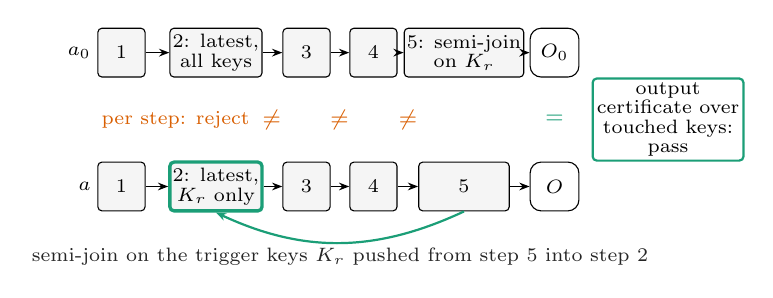
\begin{tikzpicture}[
    font=\scriptsize,
    st/.style={draw, rounded corners=1.5pt, fill=black!4, inner sep=1pt,
               minimum height=0.62cm, minimum width=0.6cm, align=center},
    wide/.style={st, minimum width=1.15cm},
    moved/.style={wide, draw=bwA, very thick},
    outn/.style={draw, rounded corners=4pt, fill=white, inner sep=1pt,
                 minimum height=0.62cm, minimum width=0.62cm},
    flow/.style={-{Stealth[length=1.3mm]}, semithick},
  ]
  % Baseline a_0, above.
  \node[anchor=east, inner sep=1pt] at (0.4,2.95) {$a_0$};
  \node[st]    (top1) at (0.75,2.95) {1};
  \node[wide]  (top2) at (1.95,2.95) {2: latest,\\[-1pt]all keys};
  \node[st]    (top3) at (3.10,2.95) {3};
  \node[st]    (top4) at (3.95,2.95) {4};
  \node[wide]  (top5) at (5.10,2.95) {5: semi-join\\[-1pt]on $K_r$};
  \node[outn]  (topO) at (6.25,2.95) {$O_0$};
  % Candidate a, below.
  \node[anchor=east, inner sep=1pt] at (0.4,1.25) {$a$};
  \node[st]    (bot1) at (0.75,1.25) {1};
  \node[moved] (bot2) at (1.95,1.25) {2: latest,\\[-1pt]$K_r$ only};
  \node[st]    (bot3) at (3.10,1.25) {3};
  \node[st]    (bot4) at (3.95,1.25) {4};
  \node[wide]  (bot5) at (5.10,1.25) {5};
  \node[outn]  (botO) at (6.25,1.25) {$O$};
  \foreach \r in {top, bot} {
    \draw[flow] (\r1) -- (\r2);
    \draw[flow] (\r2) -- (\r3);
    \draw[flow] (\r3) -- (\r4);
    \draw[flow] (\r4) -- (\r5);
    \draw[flow] (\r5) -- (\r O);
  }
  % Intermediate outputs differ: a per-step check rejects the candidate.
  \foreach \x in {2.66,3.52,4.39} {
    \node[text=bwB, font=\footnotesize] at (\x,2.1) {$\neq$};
  }
  \node[text=bwB, anchor=east, inner sep=1pt] at (2.42,2.1) {per step: reject};
  % Pipeline outputs agree over the touched keys: the certificate passes.
  \node[text=bwA, font=\footnotesize] at (6.25,2.1) {$=$};
  \node[draw=bwA, thick, rounded corners=1.5pt, fill=white, inner sep=1.5pt,
        align=center, anchor=west] at (6.72,2.1)
    {output\\[-1pt]certificate over\\[-1pt]touched keys:\\[-1pt]pass};
  % The move.
  \draw[flow, bwA, thick] (bot5.south) to[out=-155, in=-25]
    node[pos=0.5, below, inner sep=1.5pt, text=bwInk]
      {semi-join on the trigger keys $K_r$ pushed from step 5 into step 2}
    (bot2.south);
\end{tikzpicture}%

  \caption{Schematic; no measured quantities. The candidate moves step five's
    semi-join on the trigger keys into step two, as a temporal \emph{latest}
    lookup (Section~\ref{sec:nonlocal}). The outputs of steps two to four
    differ, so a per-step check rejects it; the certificate compares only the
    pipeline outputs, over the touched keys.}
  \Description{Two rows of five pipeline steps, the baseline above and the
    candidate below, joined by arrows from step to step. A curved arrow moves
    the semi-join from step five to step two. Not-equal signs mark the
    outputs of steps two to four; an equals sign and a certificate mark the
    two pipeline outputs, compared over the touched keys.}
  \label{fig:schematic-pipeline}
\end{figure}

The unit of optimization is never a single call (\adr{023}). Plans are mutated
as DAGs and scored whole, so interactions inside a plan are captured by
construction. Physical design is a set-valued configuration of key specs, a
layout, and knob values, scored by Equation~\eqref{eq:design} against every
run, with prefix-seek subsumption modeled (Section~\ref{sec:counterfactual})
and $m(a)$ kept as a separate objective. This is the classical index-selection
problem~\cite{autoadmin1997,bruno2005relax}, whose weak point was the estimate.
Search is greedy construction followed by local search with exact scoring,
seeded by rule-driven candidates and mutated by the model, and interaction terms
between key specs decide which specs are proposed together. Pipelines are DAGs
of steps with lineage; cross-step mutations are allowed and gated at the
pipeline output (Section~\ref{sec:nonlocal}; Figure~\ref{fig:schematic-pipeline}),
which is what distinguishes optimizing a pipeline from optimizing each of its
queries.

\subsection{Pareto selection over runs}\label{sec:pareto}

Scalarizing cost, for example as mean bytes over runs, hides the tail. For a
candidate $a$ let $C(a)$ be its matrix of runs by objectives, together with
$m(a)$. Candidate $a$ dominates $b$ if it is at least as good in every cell and
strictly better in one, and the frontier is the set of non-dominated members
(\doc{evolve.md} \S6). In particular, a candidate that is strictly best on any
single run survives, which is the rule stated in \adr{021}, and a candidate
that wins on the mean cannot eliminate one that protects the tail
(Figure~\ref{fig:schematic-pareto}). Crowding distance,
as in NSGA-II~\cite{nsga2}, breaks ties when choosing parents so the frontier
stays spread. Runs are grouped by template (same plan shape, different keys) so
that the frontier is not dominated by run count, and $m(a)$ is on the frontier,
so an index that saves bytes read at a large storage cost is visible rather than
hidden. Because the baseline is always in the population, the frontier never
regresses below it.

\subsection{Determinism and the ledger}\label{sec:determinism}

A search is pinned to a manifest sequence, a workload hash, a rule catalog
version, proposer identifiers, and a seed (\doc{evolve.md} \S8). Every
candidate, score, certificate, attribution, interaction matrix, frontier
snapshot, model prompt and completion, and rule is a ledger record, and the
planned contract adds a record kind for each (\code{Candidate},
\code{Attribution}, \code{Interaction}, \code{Frontier}, \code{ProposerCall},
\code{Rule}, \code{Rulebook}; \doc{evolve.md} \S10). Model outputs are not assumed to be
deterministic. Replaying a search from its ledger reuses the stored completions
and reproduces the frontier byte for byte, which extends invariant~3; a fresh
search is a new ledger. Budgets for replays, model calls, and wall-clock time
are explicit, and exhausting one is a recorded terminal state, not an error.

\subsection{The proposer in the threat model}\label{sec:proposerthreat}

Per \doc{evolve.md} \S9, a proposer may be wrong, adversarial, or compromised.
It can waste budget, propose non-equivalent artifacts, which the gate discards, and
write misleading rule text, which held-out validation rejects. It cannot score,
pass the gate, apply, or promote a rule, and a surrogate would inherit the same
limits. Because the loop invokes a language model as one of its proposers,
\adr{009}, as amended, states the boundary precisely: the engine
never consults a model for a score, a verification outcome, or an apply
decision. A proposer, model or otherwise, is invoked only to produce a Proposal
through the same path an external agent uses; its prompt and completion are
ledger records, and nothing it returns is trusted. The engine may host an
untrusted proposer, but the direction of trust is unchanged.

\subsection{The rulebook and its validation}\label{sec:rulebook}

The frontier answers for one workload; the rulebook is what transfers
(\doc{evolve.md} \S7). After a search, winning mutations are clustered by
identity and pattern, and for each cluster the model writes a rule: a detector
over evidence or plans, an action, an invariant, and the evidence hashes and
measured gains that justify it. No rule is accepted on the model's word
(\adr{025}). A rule is promoted only if applying it to held-out runs, excluded
from the search, reproduces a gain under exact replay and passes the gate.
Rules carry a confidence derived from that validation, hash links to the
evidence and receipts that produced them, and their certificates' coverage, and
a rule whose evidence has drifted is flagged stale. This is the validation gate
of SkillOpt~\cite{skillopt} applied to rules rather than skills. The rulebook is
a text artifact that agents read on the next \code{fix}, a learned analogue of
a hand-written optimization catalog, and it is the subject of the transfer
experiment in Section~\ref{sec:eval}.

\section{Implementation}\label{sec:impl}

Bellwether is a Rust workspace with one crate per work package
(\doc{work-packages.md}), each with one owner and one interface contract. The
contract crate,
\code{bellwether-types}, defines every record, trait, and format constant and
contains no logic beyond construction, hashing, and serialization; changing it
is an architectural decision. Table~\ref{tab:crates} lists the crates and their
status at the time of writing. Each crate lands by a pull request reviewed
against the invariants and decision records it owns.

\begin{table}[t]
  \caption{Crates and their status at the time of writing. \emph{Merged}: on
    the main branch. \emph{Review}: an open pull request. \emph{Planned}:
    specified, not yet written.}
  \label{tab:crates}
  \small
  \begin{tabular}{@{}l>{\raggedright\arraybackslash}p{0.53\columnwidth}l@{}}
    \toprule
    Crate & Role & Status \\
    \midrule
    types & records, traits, format constants & merged \\
    source & Parquet and chunked text sources; fingerprints & merged \\
    ledger & content-addressed records; write-time rules & merged \\
    core & canonical encoding, segments, bloom filters, bitmaps, temporal
      chains, merge & review \\
    store & conditional PUT, manifest commits, cache & review \\
    bench & synthetic ledger, workloads, harness, SLOs & review \\
    build & discovery, id assignment, segment build, compaction & planned \\
    profile & fanout, sortedness, lints, candidate composites & planned \\
    replay & workload recorder; exact replay & planned \\
    verify & reconciliation; Certificates & planned \\
    cli, mcp & one shared code path, two interfaces & planned \\
    evolve & the optimizer of Section~\ref{sec:evolve} & planned \\
    \bottomrule
  \end{tabular}
\end{table}

\paragraph{Formats.} Storage, record, and encoding formats are versioned from
the first commit, and each is at version 1 (\doc{format.md}). A binary that
meets a newer version refuses with a typed error and never downgrades in place
(\adr{017}). The canonical encoding gives each Arrow type one byte form:
integers widened to 64 bits big-endian, with the sign bit flipped for signed
types, floats under a total order with one canonical NaN, decimals rescaled to the schema's declared scale
(an unrepresentable value is an error, never rounded), escaped and terminated
strings, and timestamps normalized to UTC in the schema's unit (\adr{016}).

\paragraph{Memory bounds and budgets.} Memory is bounded per operation
(\adr{018}): a build streams one row group per worker and holds at most one
segment, whose name is the hash of its bytes; a lookup holds one block index and
the bitmaps for the keys asked; a replay holds one run's key set. Observe tools
have a 100\,ms budget (\doc{architecture.md}). For evolve on the medium
synthetic dataset, the budgets are 5\,ms per replay of one run under one
candidate, one second to attribute a 20-node plan, one minute per generation of
16 candidates excluding proposer latency, and one hour for 50 generations
(\doc{evolve.md} \S12). The harness asserts these budgets; none is a
measurement.

\paragraph{A preliminary microbenchmark.} The core crate's review branch
includes a Criterion benchmark of single-key lookup in an exact segment of
64-bit integer keys held in memory. It reports about 0.2\,\textmu s per lookup
with $10^4$ keys and about 0.5\,\textmu s with $10^6$ keys. The caveats are
material: the crate is not merged; the segment is in memory, so storage I/O,
segment open, and the manifest read are excluded; the key is a single column; no
machine description accompanies the number, although the benchmark methodology
requires one for every reported result (\doc{benchmark.md}); and in-memory
lookup latency is not one of the paper's metrics. We report the number as
context and draw no conclusion from it.

\paragraph{Interfaces.} Command-line verbs such as \code{why}, \code{fix},
\code{latest}, \code{asof}, and \code{reconcile}, with \code{evolve} and
\code{report} for the optimizer, share one code path with the MCP tiers of
Section~\ref{sec:loop} (\doc{work-packages.md}).

\section{Evaluation Methodology}\label{sec:eval}

The benchmark was designed before any implementation existed (\adr{019}), in
\doc{benchmark.md} for the index and \doc{evolve.md} \S11 for the optimizer.
A change to the design after the first harness run is recorded in
\doc{benchmark.md} with a date and a reason, and results from before the change
are labeled as such. Every dataset is synthetic; no real data is used, and none
is needed to reproduce a result. No result is reported yet
(Section~\ref{sec:results}).

\subsection{Questions}\label{sec:questions}

\textbf{Q1}: how many bytes does a keyed lookup read with the index, compared
with each baseline? \textbf{Q2}: how does lookup latency grow with corpus size?
\textbf{Q3}: how far is predicted cost from measured cost? Replay is exact by
design (\adr{005}), so the expected error is zero and any nonzero value is a
defect. \textbf{Q4}: given a planted anti-pattern, how often does the engine
recommend the fix an expert would make? \textbf{Q5}: how much does evolve reduce
cost per run at p50, p95, and max, at what maintenance cost, and with what gain
per replay and per model call? \textbf{Q6}: how many non-local rewrites does
evolve find that no local identity could certify, and do their output
certificates hold? \textbf{Q7}: what gain do promoted rules alone yield on
held-out query templates? \textbf{Q8}: does Pareto selection protect the p95
run relative to mean selection?

\subsection{Dataset}\label{sec:dataset}

The generator produces a synthetic versioned ledger: each entity has a true id
and a series of versions over time. Files are partitioned by day and written in
arrival order, so a version's location depends on when it arrived, not on its
entity, which imitates a common lake shape on purpose. Columns are a true id, a
version timestamp, a batch-stamp column (a high-cardinality value assigned per
write batch and ordered with time), a partition date, decimal amounts for totals
checks, and filler columns. The parameters are the number of files, row groups
per file, rows per row group, entities, churn, days, payload width, the
presence of the batch-stamp column, the fraction of null timestamps, and a
seed; the dataset is a pure function of the parameters and the seed. The
pre-registered corpus ladder is defined by days and files per day: small is 10
days of 1 file (10 files, 1,000,000 entities), medium is 30 days of 4 files
(120 files, 1,000,000 entities), and large is 30 days of 32 files (960 files,
10,000,000 entities). Every rung has 8 row groups per file, 100,000 rows per
row group, a payload width of 256 bytes, and corpus seed 7
(\doc{benchmark.md}, amended), so the configuration specifies 8, 96, and 768
million rows for the three rungs. The small corpus measured 2.1\,GB on disk;
from the configuration, the medium and large corpora would hold about 30\,GB
and 240\,GB. The ladder was revised before any harness run because its first
version, 10, 100, and 1,000 files over 30 days, was inconsistent with the
generator, which writes at least one file per day. Churn is the fraction of
entities re-versioned per day, 0.05. Rows per day are fixed by the layout
(files per day times 8 row groups of 100,000 rows), so from the configuration a
re-versioned entity would receive about 16, 64, and 51 versions per day on the
small, medium, and large rungs; the generator records the measured versions per
entity in its ground truth.
For evolve, the dataset adds a pipeline of several dependent steps
(\doc{evolve.md} \S11).

\paragraph{Planted anti-patterns.} A generated dataset may plant one or more
patterns from the rule catalog and records which ones it planted, as ground
truth beside the data: \code{batch\us stamp\us key} (consumer workloads join on
the batch-stamp column), \code{low\us selectivity\us single\us column} (a
declared single-column key where a composite prunes much better),
\code{declared\us but\us unused\us key} (a declared key spec that no workload
uses), and \code{scattered\us time\us column} (timestamps written out of order
across files).
The expert fix for each planted pattern is written down before the engine runs,
as part of the ground truth.

\subsection{Workloads and splits}\label{sec:workloads}

A recorded workload is a list of runs, and each run is a key set. Key-set sizes
are drawn to hit three points, p50, p95, and max. The other parameters are the
number of runs, the key skew (uniform or skewed draws from entities), the
recency bias (how strongly runs prefer recently changed entities), the mix of
\code{locate}, \code{latest}, and \code{asof} queries, and a seed. The
pre-registered workload has 200 recorded runs with key-set sizes of 50, 10,000,
and 100,000 at p50, p95, and max, split by run id into 150 search runs and 50
held-out runs that never enter the search, with workload seed 11
(\doc{benchmark.md}, amended; \doc{evolve.md} \S11). Runs are grouped by
template, and rule transfer is measured on held-out templates (\doc{evolve.md}
\S7).

\subsection{Baselines}\label{sec:baselines}

For lookups (\adr{019}): a raw scan that reads every row group and filters;
DuckDB running the same lookup as a query over the same files; Parquet-native
statistics, which prune with footer minimum and maximum values and any embedded
bloom filters but no sidecar index; and Apache DataFusion~\cite{datafusion}, a popular Rust engine that prunes with statistics, the page index, and embedded bloom filters. For evolve
(\doc{evolve.md} \S11): no index; Parquet statistics; DuckDB; DataFusion; an LLM-only
rewriter without replay, in the shape of GenRewrite~\cite{genrewrite}; and an
estimate-based advisor that uses a DuckDB or DataFusion cost estimate in place
of a what-if interface. Each baseline answers the same lookups on the same files
and must return the same rows as the engine. A baseline that returns different
rows is a failed run, not a data point (\doc{benchmark.md}).

\subsection{Metrics}\label{sec:metrics}

\emph{Bytes read} is measured: the harness wraps the file reader in a
byte-counting layer and records the compressed bytes actually fetched for each
run, alongside the planned bytes computed from row-group statistics
(\doc{benchmark.md}, amended). \emph{Latency versus corpus size} is the wall
time per lookup across the corpus ladder, at p50, p95, and max. An engine
baseline whose planning itself scans key columns, as Apache DataFusion's
pruning does, reports planning and execution latency separately, and realized
bytes for every strategy are counted by the harness's own reader, so an
engine's internal reads count the same way as the index's (\doc{benchmark.md},
amended).
\emph{Cost-estimation error} is
$|\mathit{predicted} - \mathit{measured}| / \mathit{measured}$, where
\emph{predicted} is the planned bytes and \emph{measured} is the counted bytes. \emph{Expert-fix recovery} is the fraction of planted anti-patterns for
which the top recommendation equals the recorded expert fix. Peak resident
memory per operation and observe-tool latency are recorded for the assertions of
\adr{018} (\doc{benchmark.md}). For evolve (\doc{evolve.md} \S11): cost
reduction per run at p50, p95, and max, with $m(a)$; blind recovery of planted
anti-patterns; realized versus predicted cost, zero for evolve by construction
and measured for the estimate-based baseline; gain per replay and per model
call; non-local rewrites found and whether their certificates held; transfer
gain from promoted rules on held-out templates; and p95 cost under Pareto versus
mean selection.

\paragraph{Planned versus measured bytes.} The realized-versus-predicted figure
plots the two byte counts against each other. The claim of no estimation error
means that their difference is zero for every strategy whose plan is executed as
written; any nonzero difference is reported, not hidden (\doc{benchmark.md},
amended). Section~\ref{sec:exact} lists the reads that a Replay does not count.

\subsection{Ablations}\label{sec:ablations}

Three ablations isolate the parts of evolve (\doc{evolve.md} \S11). Pareto
versus mean selection uses the same proposer budget and seed in both arms. The
attribution ablation replaces the exact per-node differences with the
proposer's self-reported attribution, holding everything else fixed
(\doc{benchmark.md}, amended). The gate ablation runs the search with and
without the gate; in the ungated arm every frontier member is reconciled after
the search, so the number of non-equivalent candidates the gate would have
rejected can be reported. That last detail is this paper's operationalization
and is not yet recorded in \doc{benchmark.md}.

\subsection{Environment and reproducibility}\label{sec:env}

Every result records the commit hash, the \code{rustc} version, the operating
system, the CPU model, the core count, memory, the storage kind (local disk, or
an object store and its region), and whether caches were warm or cold. Cold runs
drop the operating system's page cache before each lookup where the platform
allows; otherwise the result is labeled warm (\doc{benchmark.md}). A
configuration file holds every parameter, including seeds, and the harness
writes one JSON object per baseline and lookup. Charts are rendered from ledger
records by \code{bellwether report}, never edited by hand and never recomputed
for display (\doc{evolve.md} \S11), and a search can be replayed from its ledger
(Section~\ref{sec:determinism}).

\subsection{Results (pending)}\label{sec:results}

No result is reported yet. The harness has so far run only the small rung, on
one developer machine; no medium or large result exists, and a result shown
here will name its rung and machine. Tables~\ref{tab:lookup}
to~\ref{tab:ablation} and
Figures~\ref{fig:results-lookup} to~\ref{fig:results-loss} are the reporting
templates. Every table cell reads \emph{pending}. Every figure panel is a
pgfplots template over one CSV file, whose schema is fixed in
\doc{paper/data/README.md} and which \code{bellwether report -{}-paper}
writes from ledger records; a panel draws its file when the file exists and a
framed placeholder of the same size until then, so no panel is drawn from
anything but that file.

\begin{table*}[t]
  \caption{Lookup benchmark (Q1, Q2): bytes read and latency per lookup at the
    workload's p50, p95, and max key-set sizes, and peak resident memory.
    Pending: produced by \code{bellwether report} from ledger records.}
  \label{tab:lookup}
  \small
  \begin{tabular}{@{}lccccccc@{}}
    \toprule
    & \multicolumn{3}{c}{Bytes read} & \multicolumn{3}{c}{Latency} & Peak \\
    \cmidrule(lr){2-4} \cmidrule(lr){5-7}
    Method & p50 & p95 & max & p50 & p95 & max & memory \\
    \midrule
    Raw scan                & \pend & \pend & \pend & \pend & \pend & \pend & \pend \\
    Parquet statistics      & \pend & \pend & \pend & \pend & \pend & \pend & \pend \\
    DuckDB                  & \pend & \pend & \pend & \pend & \pend & \pend & \pend \\
    DataFusion              & \pend & \pend & \pend & \pend & \pend & \pend & \pend \\
    Bellwether index        & \pend & \pend & \pend & \pend & \pend & \pend & \pend \\
    \bottomrule
  \end{tabular}
\end{table*}

\begin{table*}[t]
  \caption{Evolve against baselines (Q5): bytes read per run at p50, p95, and
    max, and maintenance cost $m(a)$. Pending: produced by
    \code{bellwether report} from ledger records.}
  \label{tab:evolve}
  \small
  \begin{tabular}{@{}lccccc@{}}
    \toprule
    & \multicolumn{3}{c}{Bytes read per run} & \multicolumn{2}{c}{Maintenance $m(a)$} \\
    \cmidrule(lr){2-4} \cmidrule(lr){5-6}
    Method & p50 & p95 & max & Index bytes & Build time \\
    \midrule
    No index                          & \pend & \pend & \pend & \pend & \pend \\
    Parquet statistics                & \pend & \pend & \pend & \pend & \pend \\
    DataFusion                        & \pend & \pend & \pend & \pend & \pend \\
    DuckDB                            & \pend & \pend & \pend & \pend & \pend \\
    LLM-only rewriter (no replay)     & \pend & \pend & \pend & \pend & \pend \\
    Estimate-based advisor            & \pend & \pend & \pend & \pend & \pend \\
    Evolve                            & \pend & \pend & \pend & \pend & \pend \\
    \bottomrule
  \end{tabular}
\end{table*}

\begin{table}[t]
  \caption{Planted anti-patterns (Q4): the after shape from the rule catalog,
    and whether the top recommendation of \code{fix}, and of evolve run blind,
    equals the recorded expert fix. Pending.}
  \label{tab:recovery}
  \small
  \begin{tabular}{@{}>{\raggedright\arraybackslash}p{0.36\columnwidth}%
      >{\raggedright\arraybackslash}p{0.27\columnwidth}cc@{}}
    \toprule
    Pattern & Catalog after shape & \code{fix} & Evolve \\
    \midrule
    \code{batch\_stamp\_key} & join on the true key & \pend & \pend \\
    \code{low\_selectivity\_\allowbreak single\_column} & composite key &
      \pend & \pend \\
    \code{declared\_but\_\allowbreak unused\_key} & spec removed & \pend &
      \pend \\
    \code{scattered\_time\_\allowbreak column} & clustered by time & \pend &
      \pend \\
    \bottomrule
  \end{tabular}
\end{table}

\begin{table}[t]
  \caption{Cost-estimation error (Q3), non-local rewrites (Q6), and rulebook
    transfer (Q7). Pending.}
  \label{tab:error}
  \small
  \begin{tabular}{@{}>{\raggedright\arraybackslash}p{0.43\columnwidth}ccc@{}}
    \toprule
    Cost-estimation error on bytes & p50 & p95 & max \\
    \midrule
    Replay, lookups            & \pend & \pend & \pend \\
    Replay, evolve candidates  & \pend & \pend & \pend \\
    Estimate-based advisor     & \pend & \pend & \pend \\
    \midrule
    Rewrites and rules & \multicolumn{3}{c}{Count} \\
    \midrule
    Non-local rewrites that no local identity certifies
      & \multicolumn{3}{c}{\pend} \\
    Of these, output certificate held & \multicolumn{3}{c}{\pend} \\
    Non-equivalent candidates admitted without the gate
      & \multicolumn{3}{c}{\pend} \\
    Rules promoted after held-out validation & \multicolumn{3}{c}{\pend} \\
    \midrule
    Transfer gain from rules alone & p50 & p95 & max \\
    \midrule
    Held-out templates & \pend & \pend & \pend \\
    \bottomrule
  \end{tabular}
\end{table}

\begin{table}[t]
  \caption{Ablations (Q5, Q8): p95 bytes per run, gain per replay, and gain per
    model call. Pending.}
  \label{tab:ablation}
  \small
  \begin{tabular}{@{}lccc@{}}
    \toprule
    Variant & p95 bytes & Gain/replay & Gain/call \\
    \midrule
    Evolve (full)          & \pend & \pend & \pend \\
    Mean selection         & \pend & \pend & \pend \\
    Without attribution    & \pend & \pend & \pend \\
    Without the gate       & \pend & \pend & \pend \\
    \bottomrule
  \end{tabular}
\end{table}

\begin{figure*}[t]
  \centering
  \begin{subfigure}[t]{0.32\textwidth}
    \centering
    % Panel: the pruning funnel of one recorded run, one group of bars per
% strategy. Data: data/funnel.csv; schema in data/README.md.
\IfFileExists{data/funnel.csv}{%
  \begingroup\bwdatacatcodes
  % The rung the run was measured on, for the axis label.
  \pgfplotstableread{data/funnel.csv}\bwfunneltable
  \pgfplotstablegetelem{0}{files}\of\bwfunneltable
  \let\bwfunnelfiles\pgfplotsretval
  \begin{bwpanel}{4.1cm}
    \begin{axis}[bw, bw box={4.1cm}{0.95cm}{0.85cm}{0.12cm}{0.62cm},
        ybar=0pt, bar width=3.6pt, ymode=log, log origin=infty,
        xmin=-0.55, xmax=4.55, restrict x to domain=-0.5:4.5,
        xtick={0,...,4}, xmajorgrids=false,
        xticklabels={{raw\\scan}, {Parquet\\statistics}, {DuckDB}, {Data-\\Fusion},
          {Bell-\\wether}},
        xticklabel style={align=center},
        ylabel={row groups (\bwfunnelfiles\ files)},
        legend columns=-1, bw bar legend,
        every axis plot/.append style={draw=white, line width=0.3pt}]
      \addplot[fill=bwStageA]
        table[x expr=\bwstrategypos{\thisrow{strategy}}, y=rg_total] {data/funnel.csv};
      \addlegendentry{corpus}
      \addplot[fill=bwStageB]
        table[x expr=\bwstrategypos{\thisrow{strategy}}, y=rg_stats] {data/funnel.csv};
      \addlegendentry{after statistics}
      \addplot[fill=bwStageC]
        table[x expr=\bwstrategypos{\thisrow{strategy}}, y=rg_index] {data/funnel.csv};
      \addlegendentry{after index}
    \end{axis}
  \end{bwpanel}%
  \endgroup
}{%
  \pendingfigure[\scriptsize]{4.1cm}{the pruning funnel of one recorded run,
    as row groups in the corpus, after statistics, and after the index, per
    strategy}{funnel}%
}%

    \caption{Pruning funnel of one run (Q1).}
    \label{fig:funnel}
  \end{subfigure}\hfill
  \begin{subfigure}[t]{0.32\textwidth}
    \centering
    % Panel: lookup latency versus corpus size, one line per strategy at p50 with
% a band to p95. Data: data/latency.csv; schema in data/README.md.
\IfFileExists{data/latency.csv}{%
  \begingroup\bwdatacatcodes
  \begin{bwpanel}{4.1cm}
    \begin{axis}[bw, bw box={4.1cm}{0.95cm}{0.85cm}{0.12cm}{0.62cm},
        xmode=log, ymode=log, xmin=7, xmax=1400,
        xtick={10,120,960}, xticklabels={10,120,960},
        xlabel={files in corpus}, ylabel={latency per lookup (ms)},
        legend columns=3]
      \bwlatencyseries{index}{Bellwether}
      \bwlatencyseries{stats}{Parquet stats}
      \bwlatencyseries{datafusion}{DataFusion}
      \bwlatencyseries{duckdb}{DuckDB}
      \bwlatencyseries{raw}{raw scan}
    \end{axis}
  \end{bwpanel}%
  \endgroup
}{%
  \pendingfigure[\scriptsize]{4.1cm}{lookup latency versus corpus size per
    strategy, at p50 with a band to p95}{latency}%
}%

    \caption{Latency versus corpus size (Q2).}
    \label{fig:latency}
  \end{subfigure}\hfill
  \begin{subfigure}[t]{0.32\textwidth}
    \centering
    % Panel: measured versus predicted bytes per run, one marker series per
% strategy, with the line y = x. Data: data/realized.csv; schema in
% data/README.md.
\IfFileExists{data/realized.csv}{%
  \begingroup\bwdatacatcodes
  \bwloglimits{data/realized.csv}{predicted_bytes}{realized_bytes}%
  \begin{bwpanel}{4.1cm}
    \begin{axis}[bw, bw box={4.1cm}{0.95cm}{0.85cm}{0.12cm}{0.62cm},
        xmode=log, ymode=log,
        xmin=\bwlo, xmax=\bwhi, ymin=\bwlo, ymax=\bwhi,
        xlabel={predicted bytes}, ylabel={measured bytes},
        legend columns=-1]
      \addplot[bwAxis, line width=0.5pt, mark=none, forget plot]
        coordinates {(\bwlo,\bwlo) (\bwhi,\bwhi)};
      \addplot[bwA, only marks, mark=o, bw only={strategy}{index}]
        table[x=predicted_bytes, y=realized_bytes] {data/realized.csv};
      \addlegendentry{replay, lookups}
      \addplot[bwC, only marks, mark=triangle, bw only={strategy}{evolve}]
        table[x=predicted_bytes, y=realized_bytes] {data/realized.csv};
      \addlegendentry{replay, evolve}
      \addplot[bwB, only marks, mark=square, bw only={strategy}{estimate}]
        table[x=predicted_bytes, y=realized_bytes] {data/realized.csv};
      \addlegendentry{estimate}
    \end{axis}
  \end{bwpanel}%
  \endgroup
}{%
  \pendingfigure[\scriptsize]{4.1cm}{measured versus predicted bytes per run,
    per strategy, with the diagonal}{realized}%
}%

    \caption{Realized versus predicted bytes (Q3).}
    \label{fig:realized}
  \end{subfigure}
  \caption{Lookup and exactness. (a)~Row groups in the corpus, left after
    footer statistics and embedded bloom filters, and left after the sidecar
    index, for the search run at the workload's p95 key-set size on the
    largest rung run so far, whose size the axis label gives; a strategy
    without a stage passes its count through. (b)~Wall time per lookup,
    planning included: p50, with a band and a whisker up to p95. (c)~Measured
    against predicted bytes per run, with the line $y = x$; by design, replay
    lies on it, and a point off it is a defect, not noise. Every panel in
    Figures~\ref{fig:results-lookup} to~\ref{fig:results-loss} is drawn by
    pgfplots from a CSV file that \code{bellwether report -{}-paper} writes
    from ledger records (\doc{paper/data/README.md}); a framed box stands in
    for a panel whose file does not exist yet.}
  \Description{Three panels. (a) A grouped bar chart with a logarithmic axis of
    row groups: for each of five strategies, three bars for the corpus, after
    statistics, and after the index. (b) A log-log line chart of lookup latency
    in milliseconds against the number of files, one line per strategy with a
    shaded band up to the 95th percentile. (c) A log-log scatter plot of
    measured against predicted bytes per run, one marker style per strategy,
    with the diagonal. A panel whose data file does not exist is drawn as a
    framed box that names the file.}
  \label{fig:results-lookup}
\end{figure*}

\begin{figure*}[t]
  \centering
  \begin{subfigure}[t]{0.32\textwidth}
    \centering
    % Panel: convergence of evolve. Per generation, the best candidate so far and
% the generation's median candidate, each as its p95-run bytes (line) and a
% band from its p50-run to its max-run bytes. Data: data/convergence.csv;
% schema in data/README.md.
\IfFileExists{data/convergence.csv}{%
  \begingroup\bwdatacatcodes
  \begin{bwpanel}{4.1cm}
    \begin{axis}[bw, bw box={4.1cm}{0.95cm}{0.85cm}{0.12cm}{0.62cm},
        ymode=log, xlabel={generation}, ylabel={bytes per run},
        legend columns=-1]
      \addplot[name path=bwbestlo, draw=none, mark=none, forget plot]
        table[x=generation, y=best_p50] {data/convergence.csv};
      \addplot[name path=bwbesthi, draw=none, mark=none, forget plot]
        table[x=generation, y=best_max] {data/convergence.csv};
      \addplot[bwA, fill opacity=0.2, draw=none, forget plot]
        fill between[of=bwbestlo and bwbesthi];
      \addplot[name path=bwmedlo, draw=none, mark=none, forget plot]
        table[x=generation, y=median_p50] {data/convergence.csv};
      \addplot[name path=bwmedhi, draw=none, mark=none, forget plot]
        table[x=generation, y=median_max] {data/convergence.csv};
      \addplot[bwB, fill opacity=0.13, draw=none, forget plot]
        fill between[of=bwmedlo and bwmedhi];
      \addplot[bwA, solid, mark=none]
        table[x=generation, y=best_p95] {data/convergence.csv};
      \addlegendentry{best so far}
      \addplot[bwB, dashed, mark=none, unbounded coords=jump]
        table[x=generation, y=median_p95] {data/convergence.csv};
      \addlegendentry{median of generation}
    \end{axis}
  \end{bwpanel}%
  \endgroup
}{%
  \pendingfigure[\scriptsize]{4.1cm}{the best and the median candidate's cost
    per generation, with p50, p95, and max run bands}{convergence}%
}%

    \caption{Convergence (Q5).}
    \label{fig:convergence}
  \end{subfigure}\hfill
  \begin{subfigure}[t]{0.32\textwidth}
    \centering
    % Panel: Pareto frontier evolution, projected onto p50-run and p95-run bytes:
% the frontier at four generations, lighter for earlier ones, and the
% baseline. Data: data/frontier.csv; schema in data/README.md.
\IfFileExists{data/frontier.csv}{%
  \begingroup\bwdatacatcodes
  % The generation of each snapshot, for the legend.
  \pgfplotstableread{data/frontier.csv}\bwfrontiertable
  \pgfplotstableforeachcolumnelement{snapshot}\of\bwfrontiertable\as\bwsnap{%
    \pgfplotstablegetelem{\pgfplotstablerow}{generation}\of\bwfrontiertable
    \expandafter\xdef\csname bwgen\bwsnap\endcsname{\pgfplotsretval}}%
  \begin{bwpanel}{4.1cm}
    \begin{axis}[bw, bw box={4.1cm}{0.95cm}{0.85cm}{0.12cm}{0.62cm},
        xmode=log, ymode=log,
        xlabel={p50-run bytes}, ylabel={p95-run bytes},
        legend columns=-1,
        every axis plot/.append style={mark=*, mark options={solid}}]
      \addplot[bwA, opacity=0.3, bw only={snapshot}{1}]
        table[x=p50_bytes, y=p95_bytes] {data/frontier.csv};
      \addlegendentry{$g{=}\csname bwgen1\endcsname$}
      \addplot[bwA, opacity=0.53, bw only={snapshot}{2}]
        table[x=p50_bytes, y=p95_bytes] {data/frontier.csv};
      \addlegendentry{$\csname bwgen2\endcsname$}
      \addplot[bwA, opacity=0.77, bw only={snapshot}{3}]
        table[x=p50_bytes, y=p95_bytes] {data/frontier.csv};
      \addlegendentry{$\csname bwgen3\endcsname$}
      \addplot[bwA, bw only={snapshot}{4}]
        table[x=p50_bytes, y=p95_bytes] {data/frontier.csv};
      \addlegendentry{$\csname bwgen4\endcsname$}
      \addplot[bwInk, only marks, mark=star, mark size=2.4pt, line width=0.6pt,
          bw only={snapshot}{0}]
        table[x=p50_bytes, y=p95_bytes] {data/frontier.csv};
      \addlegendentry{baseline $a_0$}
    \end{axis}
  \end{bwpanel}%
  \endgroup
}{%
  \pendingfigure[\scriptsize]{4.1cm}{the Pareto frontier at four generations in
    p50-run and p95-run bytes, with the baseline}{frontier}%
}%

    \caption{Frontier evolution (Q8).}
    \label{fig:frontier}
  \end{subfigure}\hfill
  \begin{subfigure}[t]{0.32\textwidth}
    \centering
    % Panel: rulebook transfer. Held-out gain of each promoted rule applied
% alone, with its confidence as error bars, and the gain of rules 1 to i
% applied together. Data: data/transfer.csv; schema in data/README.md.
\IfFileExists{data/transfer.csv}{%
  \begingroup\bwdatacatcodes
  \begin{bwpanel}{4.1cm}
    \begin{axis}[bw, bw box={4.1cm}{1.75cm}{0.85cm}{0.12cm}{0.62cm},
        y dir=reverse, ytick=data, ymajorgrids=false,
        yticklabels from table={data/transfer.csv}{label},
        enlarge y limits={abs=0.6},
        xlabel={held-out gain (\% of bytes)},
        legend columns=-1]
      \addplot[xbar, bar width=3.6pt, fill=bwA, draw=none,
          legend image code/.code={\fill[bwA] (0cm,-0.06cm) rectangle (0.42cm,0.06cm);},
          error bars/.cd, x dir=both, x explicit,
          error bar style={bwInk, line width=0.5pt},
          error mark options={bwInk, rotate=90, mark size=1.4pt}]
        table[y=rank, x=gain_pct,
          x error plus expr=\thisrow{hi_pct}-\thisrow{gain_pct},
          x error minus expr=\thisrow{gain_pct}-\thisrow{lo_pct}]
        {data/transfer.csv};
      \addlegendentry{rule alone}
      \addplot[bwB, mark=*, mark options={solid}]
        table[y=rank, x=cumulative_pct] {data/transfer.csv};
      \addlegendentry{rules $1..i$ together}
    \end{axis}
  \end{bwpanel}%
  \endgroup
}{%
  \pendingfigure[\scriptsize]{4.1cm}{held-out gain per promoted rule, with its
    confidence, and the cumulative gain}{transfer}%
}%

    \caption{Rulebook transfer (Q7).}
    \label{fig:transfer}
  \end{subfigure}
  \caption{Search. (a)~Per generation, the best candidate so far (least
    p95-run bytes) and the generation's median candidate; lines are p95-run
    bytes and bands span p50-run to max-run bytes. (b)~The Pareto frontier at
    generations $G/4$, $G/2$, $3G/4$, and the last, $G$ (darker is later),
    projected onto p50-run and p95-run bytes, with the baseline $a_0$; the
    frontier is over every run and objective, so a member can look dominated
    in this projection. (c)~Held-out gain of each promoted rule applied alone
    (bars; error bars span its lowest to highest gain over held-out
    templates) and of rules $1$ to $i$ applied together (line).}
  \Description{Three panels. (a) A line chart of bytes per run on a
    logarithmic axis against generation, with a solid line for the best
    candidate and a dashed line for the median candidate, each with a shaded
    band. (b) A log-log plot of p95-run bytes against p50-run bytes showing
    four connected point sets, drawn lighter for earlier generations, and a
    star for the baseline. (c) A bar chart of held-out gain in percent per
    promoted rule with error bars, and a line of cumulative gain. A panel whose
    data file does not exist is drawn as a framed box that names the file.}
  \label{fig:results-search}
\end{figure*}

\begin{figure*}[t]
  \centering
  \begin{subfigure}[t]{0.27\textwidth}
    \centering
    % Panel: the loss landscape. Exact replay cost on a grid of two numeric knobs,
% bloom false-positive rate and key-count gate, as a surface in a
% three-quarter view, with the finite-difference descent path on it.
% Data: data/landscape.csv (grid) and data/descent.csv (path); schema in
% data/README.md.
\IfFileExists{data/landscape.csv}{%
  \begingroup\bwdatacatcodes
  \begin{bwpanel}{4.1cm}
    \begin{axis}[bw, bw box={4.1cm}{0.8cm}{0.65cm}{0.55cm}{0.3cm},
        view={35}{30}, xmode=log, ymode=log,
        xlabel={bloom FPR}, ylabel={key-count gate}, zlabel={bytes},
        colormap name=bwblues,
        xlabel style={sloped like x axis}, ylabel style={sloped like y axis}]
      \addplot3[surf, shader=interp, mesh/ordering=y varies]
        table[x=fpr, y=gate, z=bytes] {data/landscape.csv};
      \IfFileExists{data/descent.csv}{%
        \addplot3[bwB, mark=*, mark size=0.9pt, line width=0.7pt]
          table[x=fpr, y=gate, z=bytes] {data/descent.csv};
        \addplot3[bwB, only marks, mark=o, mark size=2pt, line width=0.6pt,
            bw only={step}{0}]
          table[x=fpr, y=gate, z=bytes] {data/descent.csv};
      }{}
    \end{axis}
  \end{bwpanel}%
  \endgroup
}{%
  \pendingfigure[\scriptsize]{4.1cm}{exact replay cost on a grid of two
    knobs as a surface, with the descent path}{landscape}%
}%

    \caption{Loss landscape and descent.}
    \label{fig:landscape}
  \end{subfigure}\hfill
  \begin{subfigure}[t]{0.235\textwidth}
    \centering
    % Panel: the same grid as data/landscape.csv as a filled contour map, with the
% descent path. Data: data/landscape.csv and data/descent.csv; schema in
% data/README.md.
\IfFileExists{data/landscape.csv}{%
  \begingroup\bwdatacatcodes
  \begin{bwpanel}{4.1cm}
    \begin{axis}[bw, bw box={4.1cm}{0.95cm}{0.92cm}{0.38cm}{0.75cm},
        view={0}{90}, xmode=log, ymode=log,
        xlabel={bloom FPR}, ylabel={key-count gate},
        colormap name=bwblues, enlargelimits=false, axis on top, grid=none,
        bw colorbar]
      \addplot3[contour filled={number=8}, mesh/ordering=y varies]
        table[x=fpr, y=gate, z=bytes] {data/landscape.csv};
      \IfFileExists{data/descent.csv}{%
        \addplot3[bwB, mark=*, mark size=0.9pt, line width=0.7pt]
          table[x=fpr, y=gate, z=bytes] {data/descent.csv};
        \addplot3[bwB, only marks, mark=o, mark size=2pt, line width=0.6pt,
            bw only={step}{0}]
          table[x=fpr, y=gate, z=bytes] {data/descent.csv};
      }{}
    \end{axis}
  \end{bwpanel}%
  \endgroup
}{%
  \pendingfigure[\scriptsize]{4.1cm}{the same grid as a contour map, with
    the descent path}{landscape}%
}%

    \caption{The same grid, contours.}
    \label{fig:contour}
  \end{subfigure}\hfill
  \begin{subfigure}[t]{0.29\textwidth}
    \centering
    % Panel: counterfactual attribution. Delta_v in bytes for each attributed
% node v of the baseline (rows) on each search run (columns), on a diverging
% scale centered on zero. Data: data/attribution.csv; schema in
% data/README.md.
\IfFileExists{data/attribution.csv}{%
  \begingroup\bwdatacatcodes
  \bwsymlimit{data/attribution.csv}{delta_bytes}%
  \bwmaxint{data/attribution.csv}{op}%
  \begin{bwpanel}{4.1cm}
    \begin{axis}[bw, bw box={4.1cm}{1.3cm}{0.92cm}{0.1cm}{0.75cm},
        colormap name=bwdiverging, point meta min=-\bwabs, point meta max=\bwabs,
        bw colorbar,
        y dir=reverse, ytick={0,...,\bwlast},
        yticklabels from table={data/attribution.csv}{label},
        xlabel={search run}, enlargelimits=false, axis on top, grid=none,
        unbounded coords=jump]
      \addplot[matrix plot*, mesh/ordering=y varies, point meta=explicit]
        table[x=run, y=op, meta=delta_bytes] {data/attribution.csv};
    \end{axis}
  \end{bwpanel}%
  \endgroup
}{%
  \pendingfigure[\scriptsize]{4.1cm}{counterfactual attribution per node and
    run}{attribution}%
}%

    \caption{Attribution $\Delta_v$.}
    \label{fig:attribution}
  \end{subfigure}\hfill
  \begin{subfigure}[t]{0.165\textwidth}
    \centering
    % Panel: pairwise interaction. I_uv in bytes, summed over search runs, for
% the nodes of the attribution panel in the same order on both axes; the
% diagonal is undefined. Data: data/interaction.csv; schema in
% data/README.md.
\IfFileExists{data/interaction.csv}{%
  \begingroup\bwdatacatcodes
  \bwsymlimit{data/interaction.csv}{i_bytes}%
  \begin{bwpanel}{4.1cm}
    \begin{axis}[bw, bw box={4.1cm}{0.2cm}{0.92cm}{0.1cm}{0.75cm},
        colormap name=bwdiverging, point meta min=-\bwabs, point meta max=\bwabs,
        bw colorbar,
        y dir=reverse, xtick distance=1, ytick distance=1,
        xticklabels={}, yticklabels={},
        xlabel={$u$, $v$: nodes of (c)}, enlargelimits=false, axis on top,
        grid=none, unbounded coords=jump,
        axis background/.style={fill=bwGrid}]
      \addplot[matrix plot*, point meta=explicit]
        table[x=v, y=u, meta=i_bytes] {data/interaction.csv};
    \end{axis}
  \end{bwpanel}%
  \endgroup
}{%
  \pendingfigure[\scriptsize]{4.1cm}{the pairwise interaction
    matrix}{interaction}%
}%

    \caption{Interaction $I_{uv}$.}
    \label{fig:interaction}
  \end{subfigure}
  \caption{The exact loss as an instrument. (a,\,b)~Exact replay bytes, the
    scalar that descent minimizes, on a grid of bloom false-positive rate and
    key-count gate, with the finite-difference descent path. This figure is
    possible only because the loss is exact and cheap enough to evaluate at
    every grid point; an estimate-based advisor has no such surface to draw.
    (c)~Attribution $\Delta_v$ (Equation~\eqref{eq:attr}) of the baseline's
    attributed nodes on each search run; red marks a node that reads more
    than its alternative would. (d)~Interaction $I_{uv}$
    (Equation~\eqref{eq:interaction}) summed over search runs; blue marks a
    pair whose joint change saves more than its two changes do separately,
    red less, and the diagonal is undefined.}
  \Description{Four panels. (a) A three-dimensional surface of bytes over two
    knobs, bloom false-positive rate and key-count gate, both on logarithmic
    axes, viewed from an oblique angle, with a descent path drawn as a line
    with markers on the surface. (b) The same grid as a filled contour map with
    the same path. (c) A heatmap of attribution in bytes with plan nodes as
    rows and search runs as columns, on a diverging blue-to-red scale. (d) A
    square heatmap of pairwise interaction in bytes on the same scale. A panel
    whose data file does not exist is drawn as a framed box that names the
    file.}
  \label{fig:results-loss}
\end{figure*}

\section{Discussion and Limitations}\label{sec:discussion}

\paragraph{Certificates are workload-scoped.} Scoping a certificate to the keys
a workload touched is what makes non-local rewrites certifiable, and it is the
main weakness: a change that is wrong only for untouched keys passes. The
design states the coverage on every Certificate, re-validates rules on held-out
runs, and records how to communicate the scope to users as an open question
(\doc{evolve.md} \S13). A full certificate closes the gap at the cost of
comparing every key.

\paragraph{The attribution cap.} Capping attribution at the top $k$ nodes by
cost keeps every reported number exact (\adr{024}) at the price of blindness: a
node outside the top $k$ receives no attribution, and an interaction between a
cheap node and an expensive one is missed if the cheap node is not attributed.

\paragraph{Rulebook overfitting.} Rules distilled from searches on a synthetic
ledger with planted patterns may learn the generator. The held-out split
mitigates this within one generator; a second generator with different patterns
is the real test, as the design notes (\doc{evolve.md} \S13).

\paragraph{Model nondeterminism.} Model outputs are not reproducible on demand,
and evolve does not assume they are: replaying a search reuses its recorded
completions (Section~\ref{sec:determinism}), so reproducibility is a property
of a recorded search, not of the model.

\paragraph{What Bellwether does not do.} It is not a query engine: it produces a
scan plan, and DuckDB, DataFusion, Polars, Spark, or user code reads the rows.
It is not a table format: it never rewrites data or asks for a conversion. It is
not a database: data that fits a relational system should use that system's
indexes. It is not an estimator: a cost it cannot compute exactly is labeled,
never guessed. It is not an autonomous agent: the model proposes, the engine
scores, verifies, applies, and records, and that direction does not reverse
(\doc{README.md}; \adr{009}).

\paragraph{Status.} Most of the system is unbuilt and every result is pending.
A measurement that contradicts a design property, such as a nonzero difference
between planned and measured bytes for a plan executed as written
(Section~\ref{sec:metrics}), will be reported as a defect in the design.

\section{Conclusion}\label{sec:conclusion}

Index advisors and language-model tuners are both limited by the estimate they
score against. A data lake exposes its files, so the I/O cost of a hypothetical
index, key, or plan over those files can be computed exactly by replaying
recorded key sets against row-group metadata. Bellwether builds on that
observation with an exact counterfactual what-if interface, reconciliation
certificates that admit non-local rewrites, a reflective optimizer whose
backward pass is counterfactual attribution and whose selection is Pareto over
recorded runs, a rulebook promoted only by held-out replay, and a boundary under
which a model proposes and only the engine scores, verifies, and applies. The
design and the evaluation are fixed; the results are pending.


\bibliographystyle{ACM-Reference-Format}
\bibliography{references}

\end{document}
